%%
%% This is file `sample-sigconf.tex',
%% generated with the docstrip utility.
%%
%% The original source files were:
%%
%% samples.dtx  (with options: `sigconf')
%% 
%% IMPORTANT NOTICE:
%% 
%% For the copyright see the source file.
%% 
%% Any modified versions of this file must be renamed
%% with new filenames distinct from sample-sigconf.tex.
%% 
%% For distribution of the original source see the terms
%% for copying and modification in the file samples.dtx.
%% 
%% This generated file may be distributed as long as the
%% original source files, as listed above, are part of the
%% same distribution. (The sources need not necessarily be
%% in the same archive or directory.)
%%
%% The first command in your LaTeX source must be the \documentclass command.
\documentclass[sigconf]{acmart}

\graphicspath{{Fig/}}

%%
%% \BibTeX command to typeset BibTeX logo in the docs
\AtBeginDocument{%
  \providecommand\BibTeX{{%
    \normalfont B\kern-0.5em{\scshape i\kern-0.25em b}\kern-0.8em\TeX}}}

%% Rights management information.  This information is sent to you
%% when you complete the rights form.  These commands have SAMPLE
%% values in them; it is your responsibility as an author to replace
%% the commands and values with those provided to you when you
%% complete the rights form.
\setcopyright{acmcopyright}
\copyrightyear{2020}
\acmYear{2020}
\acmDOI{10.1145/1122445.1122456}

%% These commands are for a PROCEEDINGS abstract or paper.
\acmConference[Woodstock '18]{Woodstock '18: ACM Symposium on Neural
  Gaze Detection}{June 03--05, 2018}{Woodstock, NY}
\acmBooktitle{Woodstock '18: ACM Symposium on Neural Gaze Detection,
  June 03--05, 2018, Woodstock, NY}
\acmPrice{15.00}
\acmISBN{978-1-4503-XXXX-X/18/06}


%%
%% Submission ID.
%% Use this when submitting an article to a sponsored event. You'll
%% receive a unique submission ID from the organizers
%% of the event, and this ID should be used as the parameter to this command.
%%\acmSubmissionID{123-A56-BU3}

%%
%% The majority of ACM publications use numbered citations and
%% references.  The command \citestyle{authoryear} switches to the
%% "author year" style.
%%
%% If you are preparing content for an event
%% sponsored by ACM SIGGRAPH, you must use the "author year" style of
%% citations and references.
%% Uncommenting
%% the next command will enable that style.
%%\citestyle{acmauthoryear}

%%
%% end of the preamble, start of the body of the document source.
\begin{document}

%%
%% The "title" command has an optional parameter,
%% allowing the author to define a "short title" to be used in page headers.
\title{Misaka: Versatile swarm robotics platform for swarm user interface development}

%%
%% The "author" command and its associated commands are used to define
%% the authors and their affiliations.
%% Of note is the shared affiliation of the first two authors, and the
%% "authornote" and "authornotemark" commands
%% used to denote shared contribution to the research.

% \author{Tingliang Zhang}
% \email{ztl20@mails.tsinghua.edu.cn}
% \orcid{0000-0002-0164-4700}
% \affiliation{%
%   \institution{Tsinghua University}
%   \streetaddress{Qinghuayuan, Haidian District}
%   \city{Beijing}
%   \country{China}
%   \postcode{100084}
% }

% \author{Haipeng Mi}
% \email{mhp@tsinghua.edu.cn}
% \affiliation{%
%   \institution{Tsinghua University}
%   \streetaddress{Qinghuayuan, Haidian District}
%   \city{Beijing}
%   \country{China}
%   \postcode{100084}
% }

%%
%% By default, the full list of authors will be used in the page
%% headers. Often, this list is too long, and will overlap
%% other information printed in the page headers. This command allows
%% the author to define a more concise list
%% of authors' names for this purpose.
\renewcommand{\shortauthors}{Tingliang and Haipeng}

%%
%% The abstract is a short summary of the work to be presented in the
%% article.
\begin{abstract}
  This paper introduces a versatile swarm robotics platform for distributed algorithm visualization, also an extendable open-source open-hardware platform for developing tabletop tangible swarm interfaces. 
  We provide two different versions of Misaka: the commercial version and the explorer version. The commercial version is Swarm robots for distributed algorithm development, while the explorer version, which is an open-source PCB, gives users more freedom to develop their own swarm interface for specific purposes.
  Bluetooth 5.1 provides us with high-bandwidth communication, as well as a new method of positioning Misaka. We will integrate it into Misaka when we get the commercial model.


\end{abstract}

%%
%% The code below is generated by the tool at http://dl.acm.org/ccs.cfm.
%% Please copy and paste the code instead of the example below.
%%
\begin{CCSXML}
  <ccs2012>
     <concept>
         <concept_id>10003120.10003123.10011760</concept_id>
         <concept_desc>Human-centered computing~Systems and tools for interaction design</concept_desc>
         <concept_significance>500</concept_significance>
         </concept>
     <concept>
         <concept_id>10010583.10010584.10010587</concept_id>
         <concept_desc>Hardware~PCB design and layout</concept_desc>
         <concept_significance>300</concept_significance>
         </concept>
   </ccs2012>
\end{CCSXML}

\ccsdesc[500]{Human-centered computing~Systems and tools for interaction design}
\ccsdesc[300]{Hardware~PCB design and layout}

%%
%% Keywords. The author(s) should pick words that accurately describe
%% the work being presented. Separate the keywords with commas.
\keywords{Swarm, tangible interface, hardware platform, Human-Robot Interaction}

%% A "teaser" image appears between the author and affiliation
%% information and the body of the document, and typically spans the
%% page.
% \begin{teaserfigure}
%   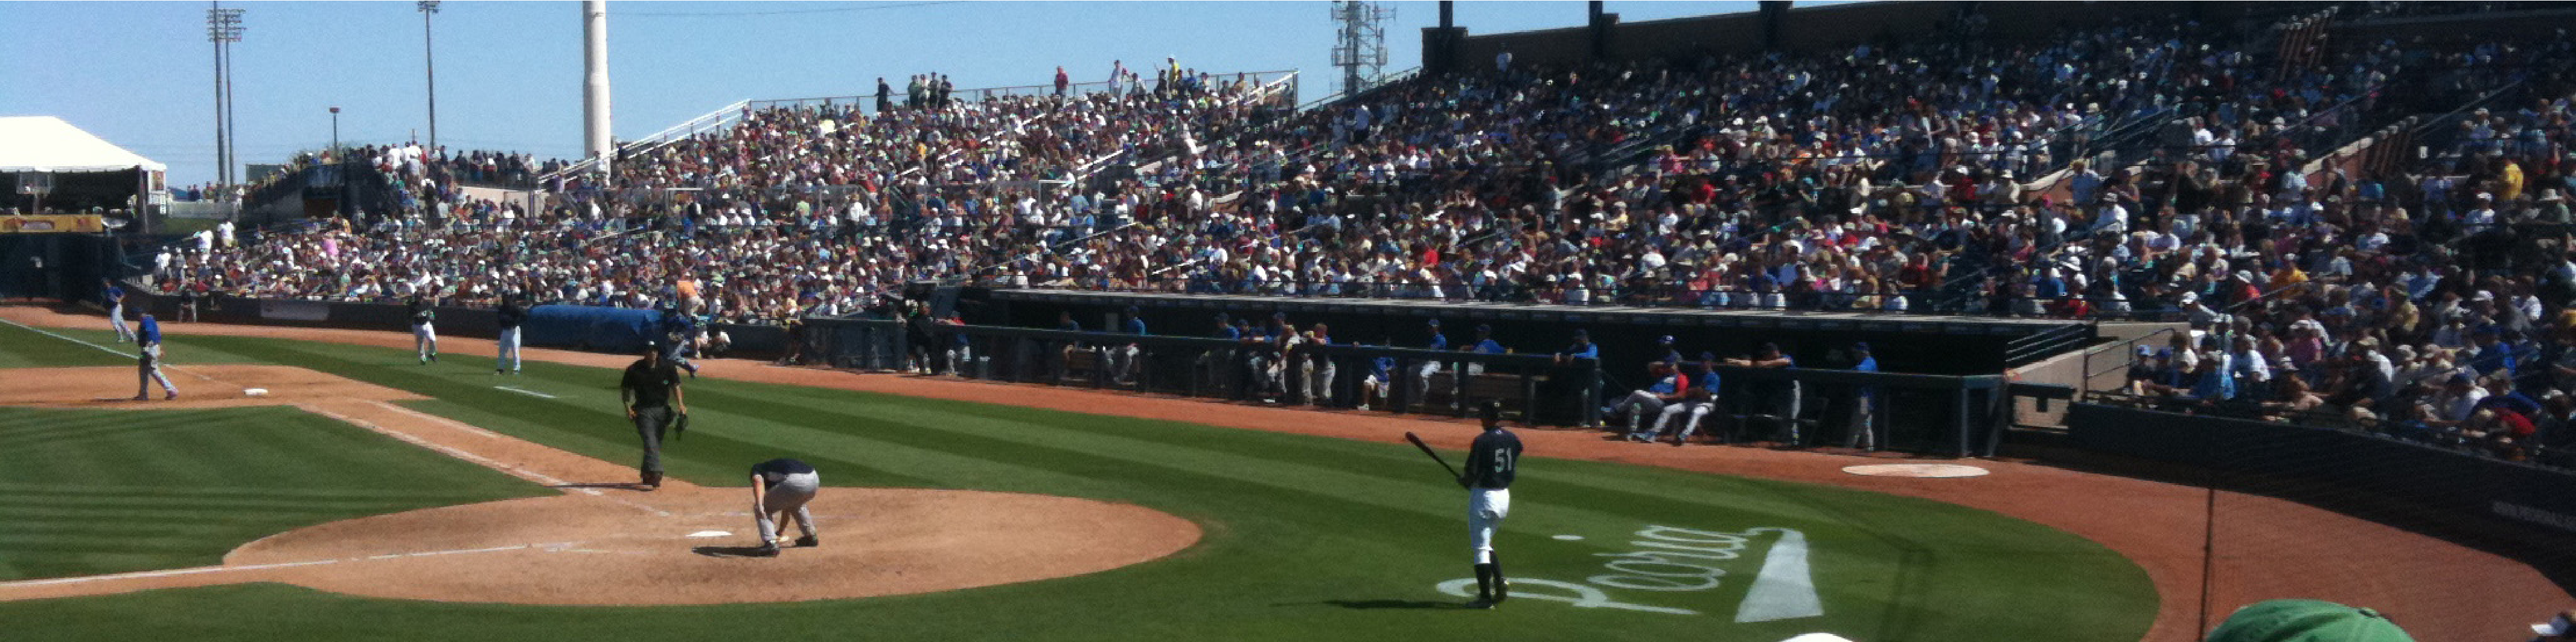
\includegraphics[width=\textwidth]{sampleteaser}
%   \caption{Seattle Mariners at Spring Training, 2010.}
%   \Description{Enjoying the baseball game from the third-base
%   seats. Ichiro Suzuki preparing to bat.}
%   \label{fig:teaser}
% \end{teaserfigure}

%%
%% This command processes the author and affiliation and title
%% information and builds the first part of the formatted document.
\maketitle

\section{Introduction}

The name of our platform, Misaka, comes from "Misaka Network" in the light novel, manga, and anime series, A Certain Magical Index, and its side-story mangas and anime series, A Certain Scientific Railgun and A Certain Scientific Accelerator. The Misaka Network is a brainwave network formed between the Sisters. The Sisters are Mikoto Misaka's 20,000 clones, who can share their thoughts and memories within their communication network. Misaka Network is actually a strongly-connected distributed network. One of our platform's typical applications is verifying distributed algorithms in a decentralized network, so we choose Misaka to be our product's name.

We design two different versions of Misaka: the commercial version and the explorer version. 

The commercial version is Swarm robots, equipped with onmi-wheels and stepper motors, and can move holonomic and precisely. Distributed algorithms researchers can utilize it as a fully decentralized hardware platform to test newly raised algorithms, also a visualization platform of all kinds of consensus algorithms. Furthermore, teachers can use it as a great tool to visualize dynamic multiple scatterplots and to explain theories to their students. 

The explorer version is for those researchers who want to develop tabletop swarm robots of their own. This version is a single PCB, which integrates almost all functionalities needed to develop any kind of swarm interface for many purposes.

Both versions have the ability to add suitable extensions to it. We also provide models adding function to it, such as computer vision, wifi, machine learning algorithms, etc.

\section{Backgroud and related work}

There are many tangible swarm robots such as Zooids\cite{le2016zooids} and Cellulo\cite{ozgur2017cellulo}. But none of them is both compact and omnidirectional.

\section{Interaction Design}

\subsection{Distributed algorithms test and visualization}

Distributed algorithm verification is mostly carried out in a pure software environment of a single device, such as Matlab simulation, which lacks a general hardware platform to test the feasibility of these algorithms in actual communication scenarios.

Most of the newly proposed algorithms are verified in a pure software environment of a single device, without considering the communication delays in the actual hardware environment, data packet order, and poor communication connections. The ZigBee chip which is used in our platform is widely used in the Internet of Things systems, and can well simulate the hardware communication environment.

This platform makes a completely decentralized test environment possible. At the same time, since this is a convenient visual development tool, it makes interactive code writing/testing/display possible. Distributed algorithm developers can use our decentralized platform to test the feasibility of the hardware and get interactive code writing, testing, and display experience.

For example, when we develop a consensus algorithm, 

\subsection{Teaching application}

Some concepts are difficult to understand, so you can use a swarm interface to do interactive and interesting teaching.

For example, a swarm system can be used to describe a scatter plot with multi-dimensional variables, etc.

% \subsection{Misaka as a learning tool}



\section{Hardware Design}

To make our hardware more universal, we design two different versions of Misaka: the commercial version and the explorer version.

\subsection{Commercial version}

The commercial version aims at HRI applications, as well as algorithms development and visualization scenarios. It is a small custom-made robot as shown in Fig{fig:CommercialVersion}.

\begin{figure}[h]
  \centering
  \includegraphics[width=\linewidth]{DA4A4015.JPG}
  \caption{The commercial version}
  \label{fig:CommercialVersion}
\end{figure}

The commercial version consists of a 3D printed frame, custom-designed PCB, battery, omni-directional wheels, and micro stepper motors.

The frame is printed using PLA(Polylactic Acid). It is carefully designed to fit the motors, wheels, and the PCB. The 3D Model of it is shown in Fig~\ref{fig:Frame}, and the CAD detail is shown in Fig~\ref{fig:CAD}.

\begin{figure}[h]
  \centering
  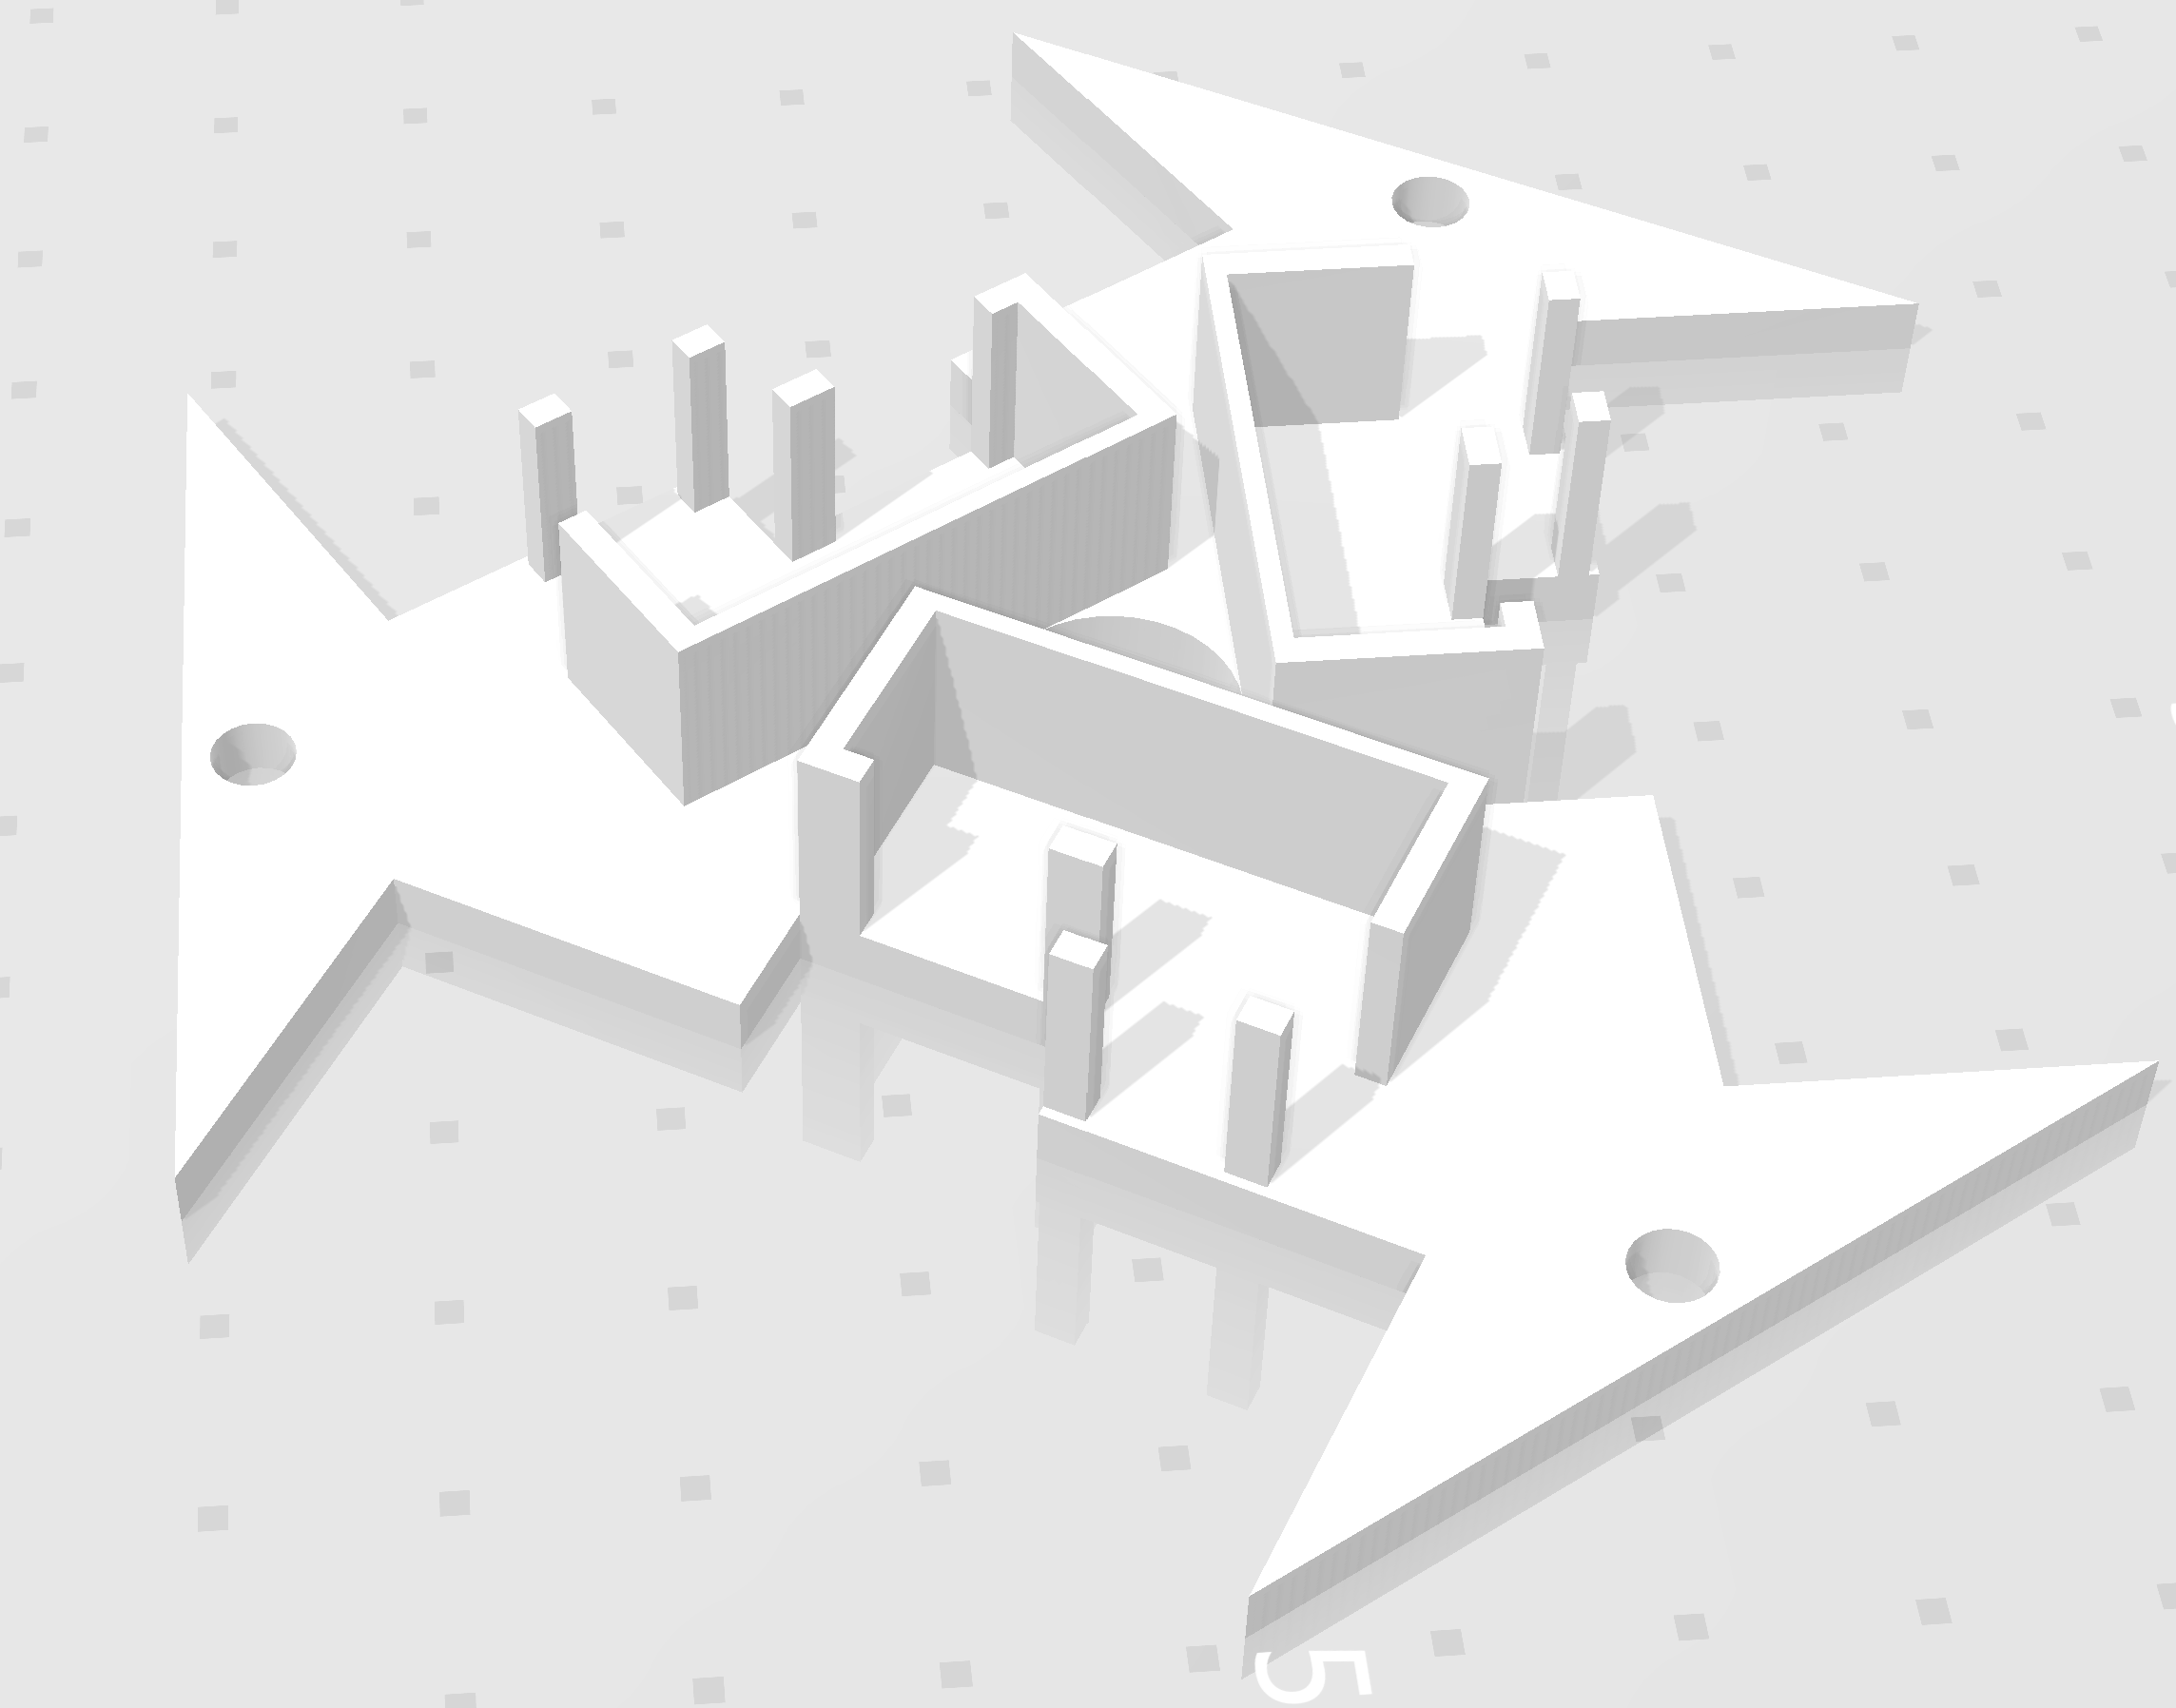
\includegraphics[width=\linewidth]{Frame.png}
  \caption{3D Model of the Frame}
  \label{fig:Frame}
\end{figure}

\begin{figure}[h]
  \centering
  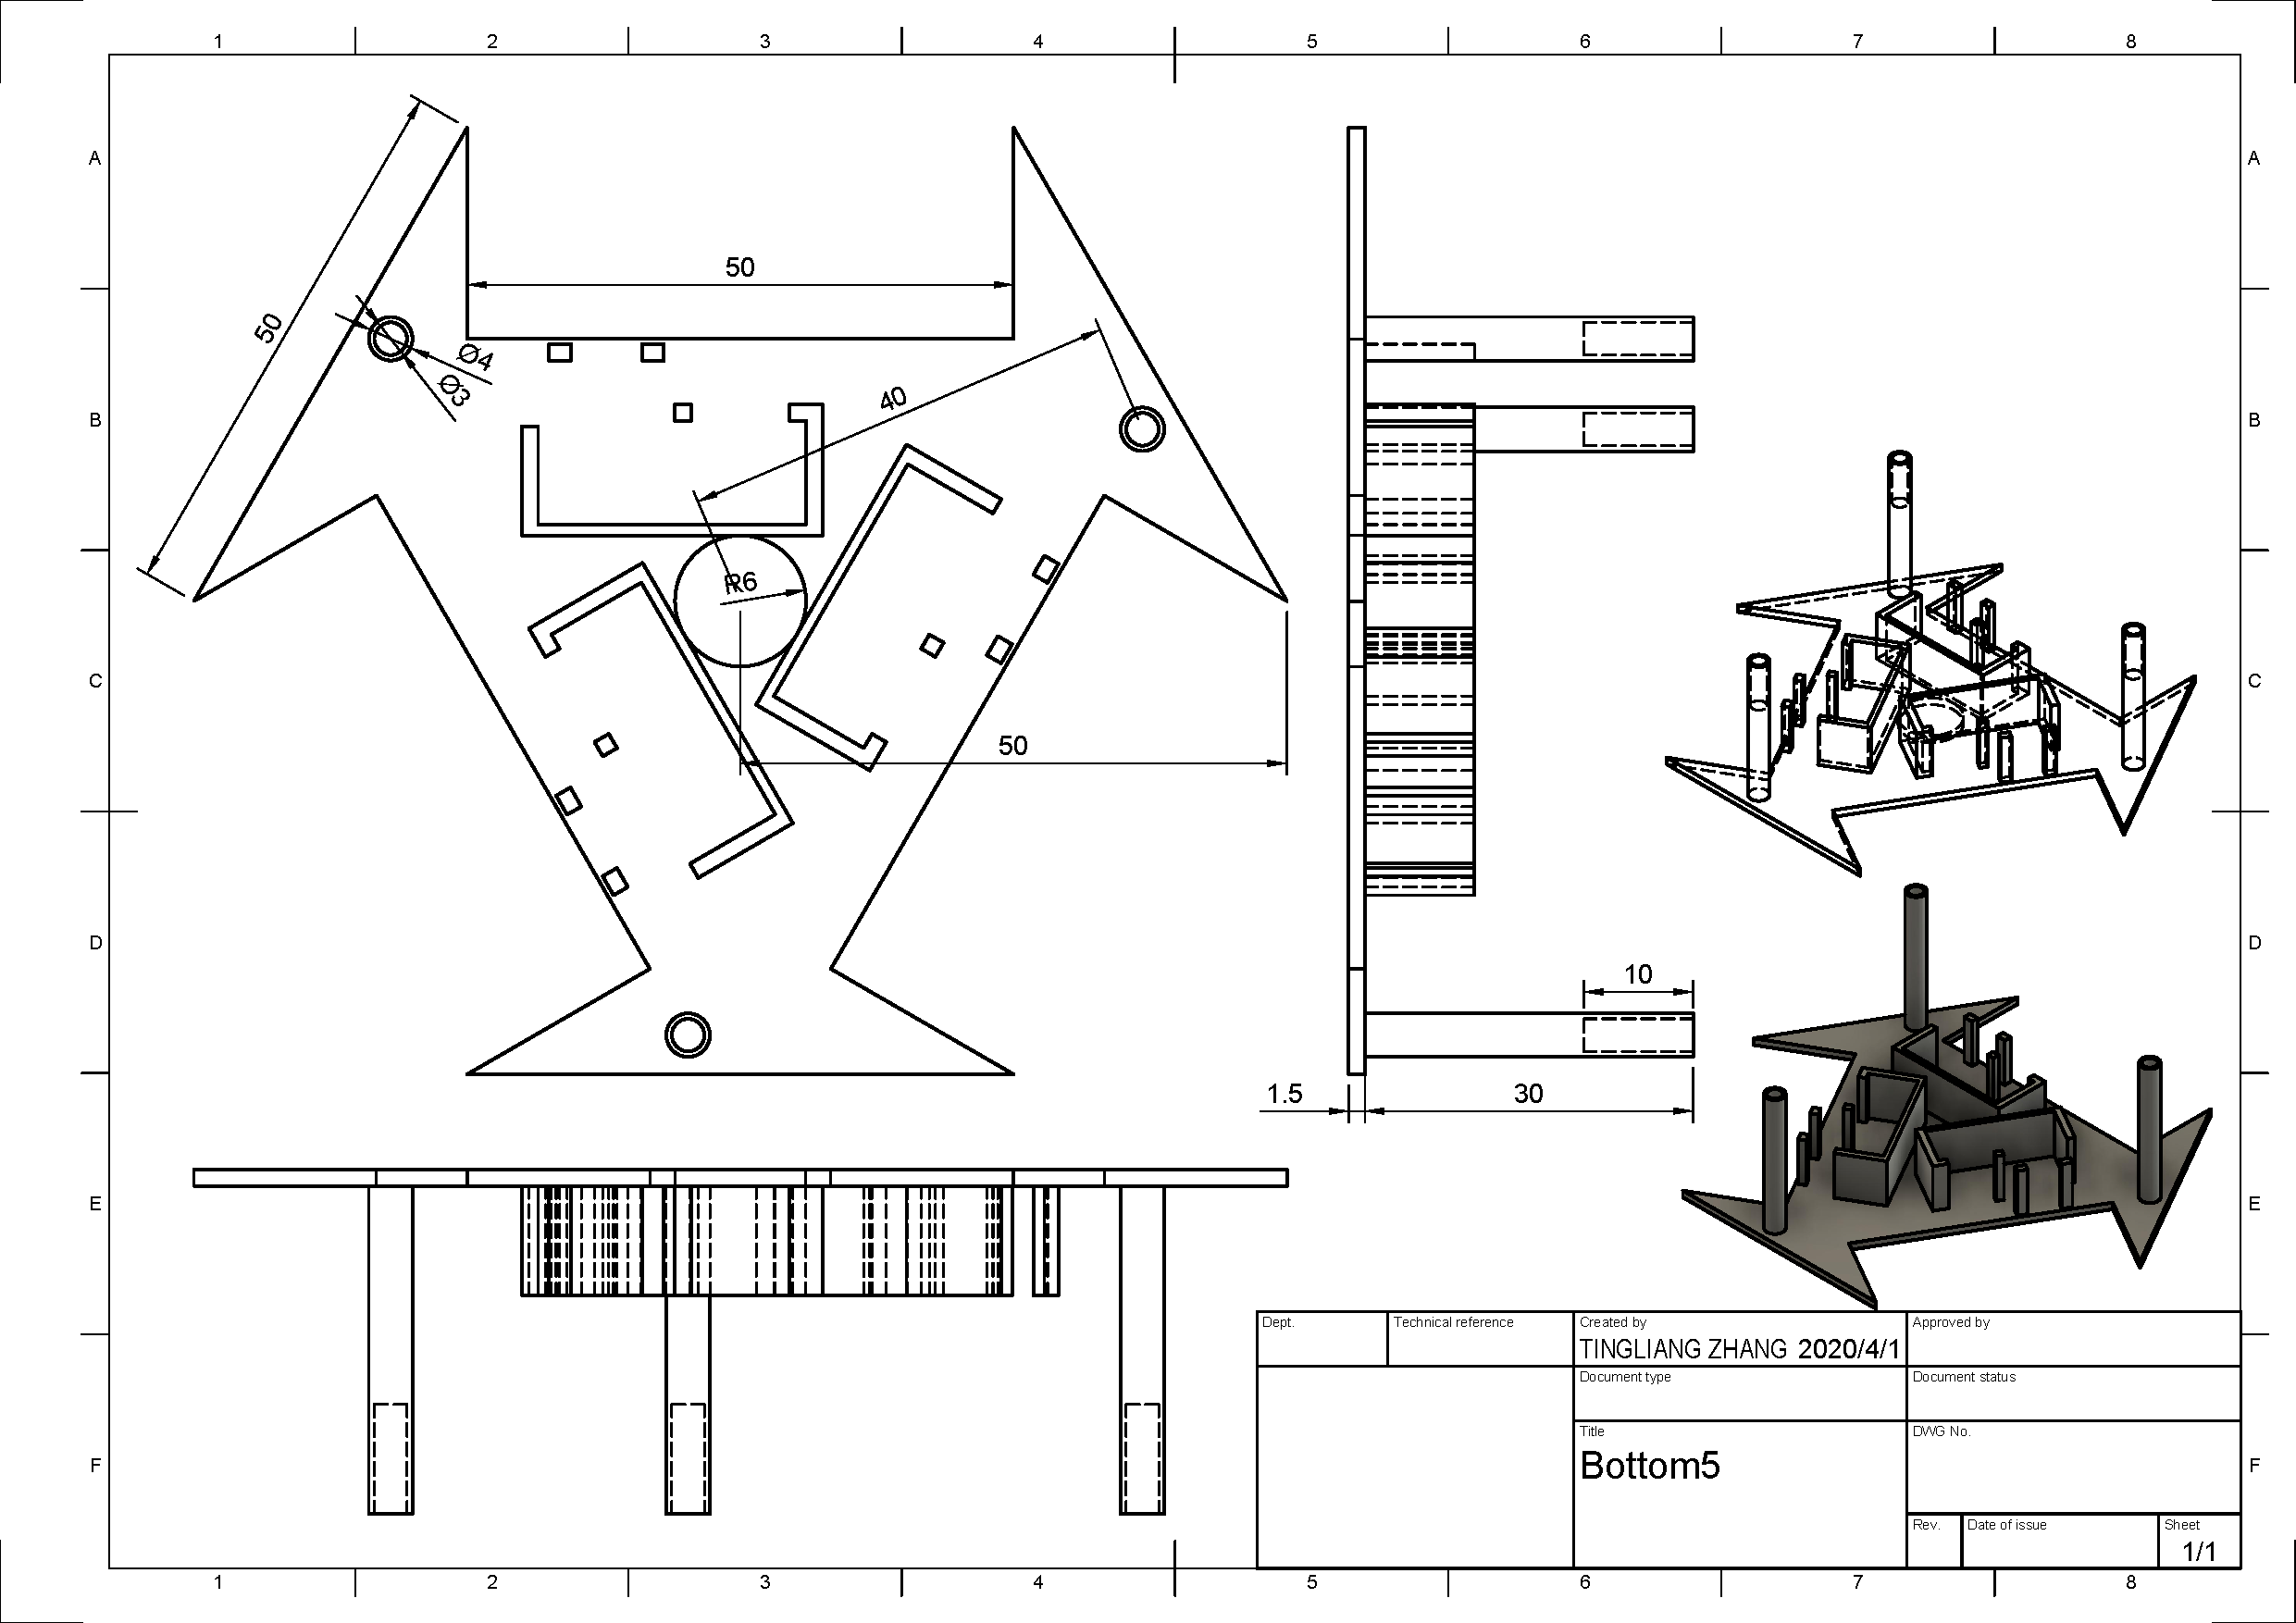
\includegraphics[width=\linewidth]{Bottom.pdf}
  \caption{the CAD of the Frame}
  \label{fig:CAD}
\end{figure}

Its dimensions are 100 mm in diameter and 50 mm in height. Each robot is powered by a 450mAh 2S 7.4V LiPo battery. Most of the power in the robots are consumed by the motors. The current draw of each robot is approximately 100 mA when the motors are stalled and 800 mA during typical use. Thus, with a 450 mAh battery, robots are capable of moving for half an hour and can work even longer with BLE(Bluetooth Low Energy). 

Three 38-mm-diameter omni-directional wheels are driven by micro stepper motors to precisely control the rotation angle of each wheel. To drive the robot, a motor driver chip (DRV8825) and three 2-phase 4-wire Stepper Gear Motor are used. With this combination, the robot has a maximum speed of approximately 20 cm/s. The holonomic system allows robots to move precisely and can easily respond to user interaction. The shape of the holonomic chassis is shown in Fig~\ref{fig:ChassisRender}, and the real picture of it is shown in Fig~\ref{fig:chassis}.

\begin{figure}[h]
  \centering
  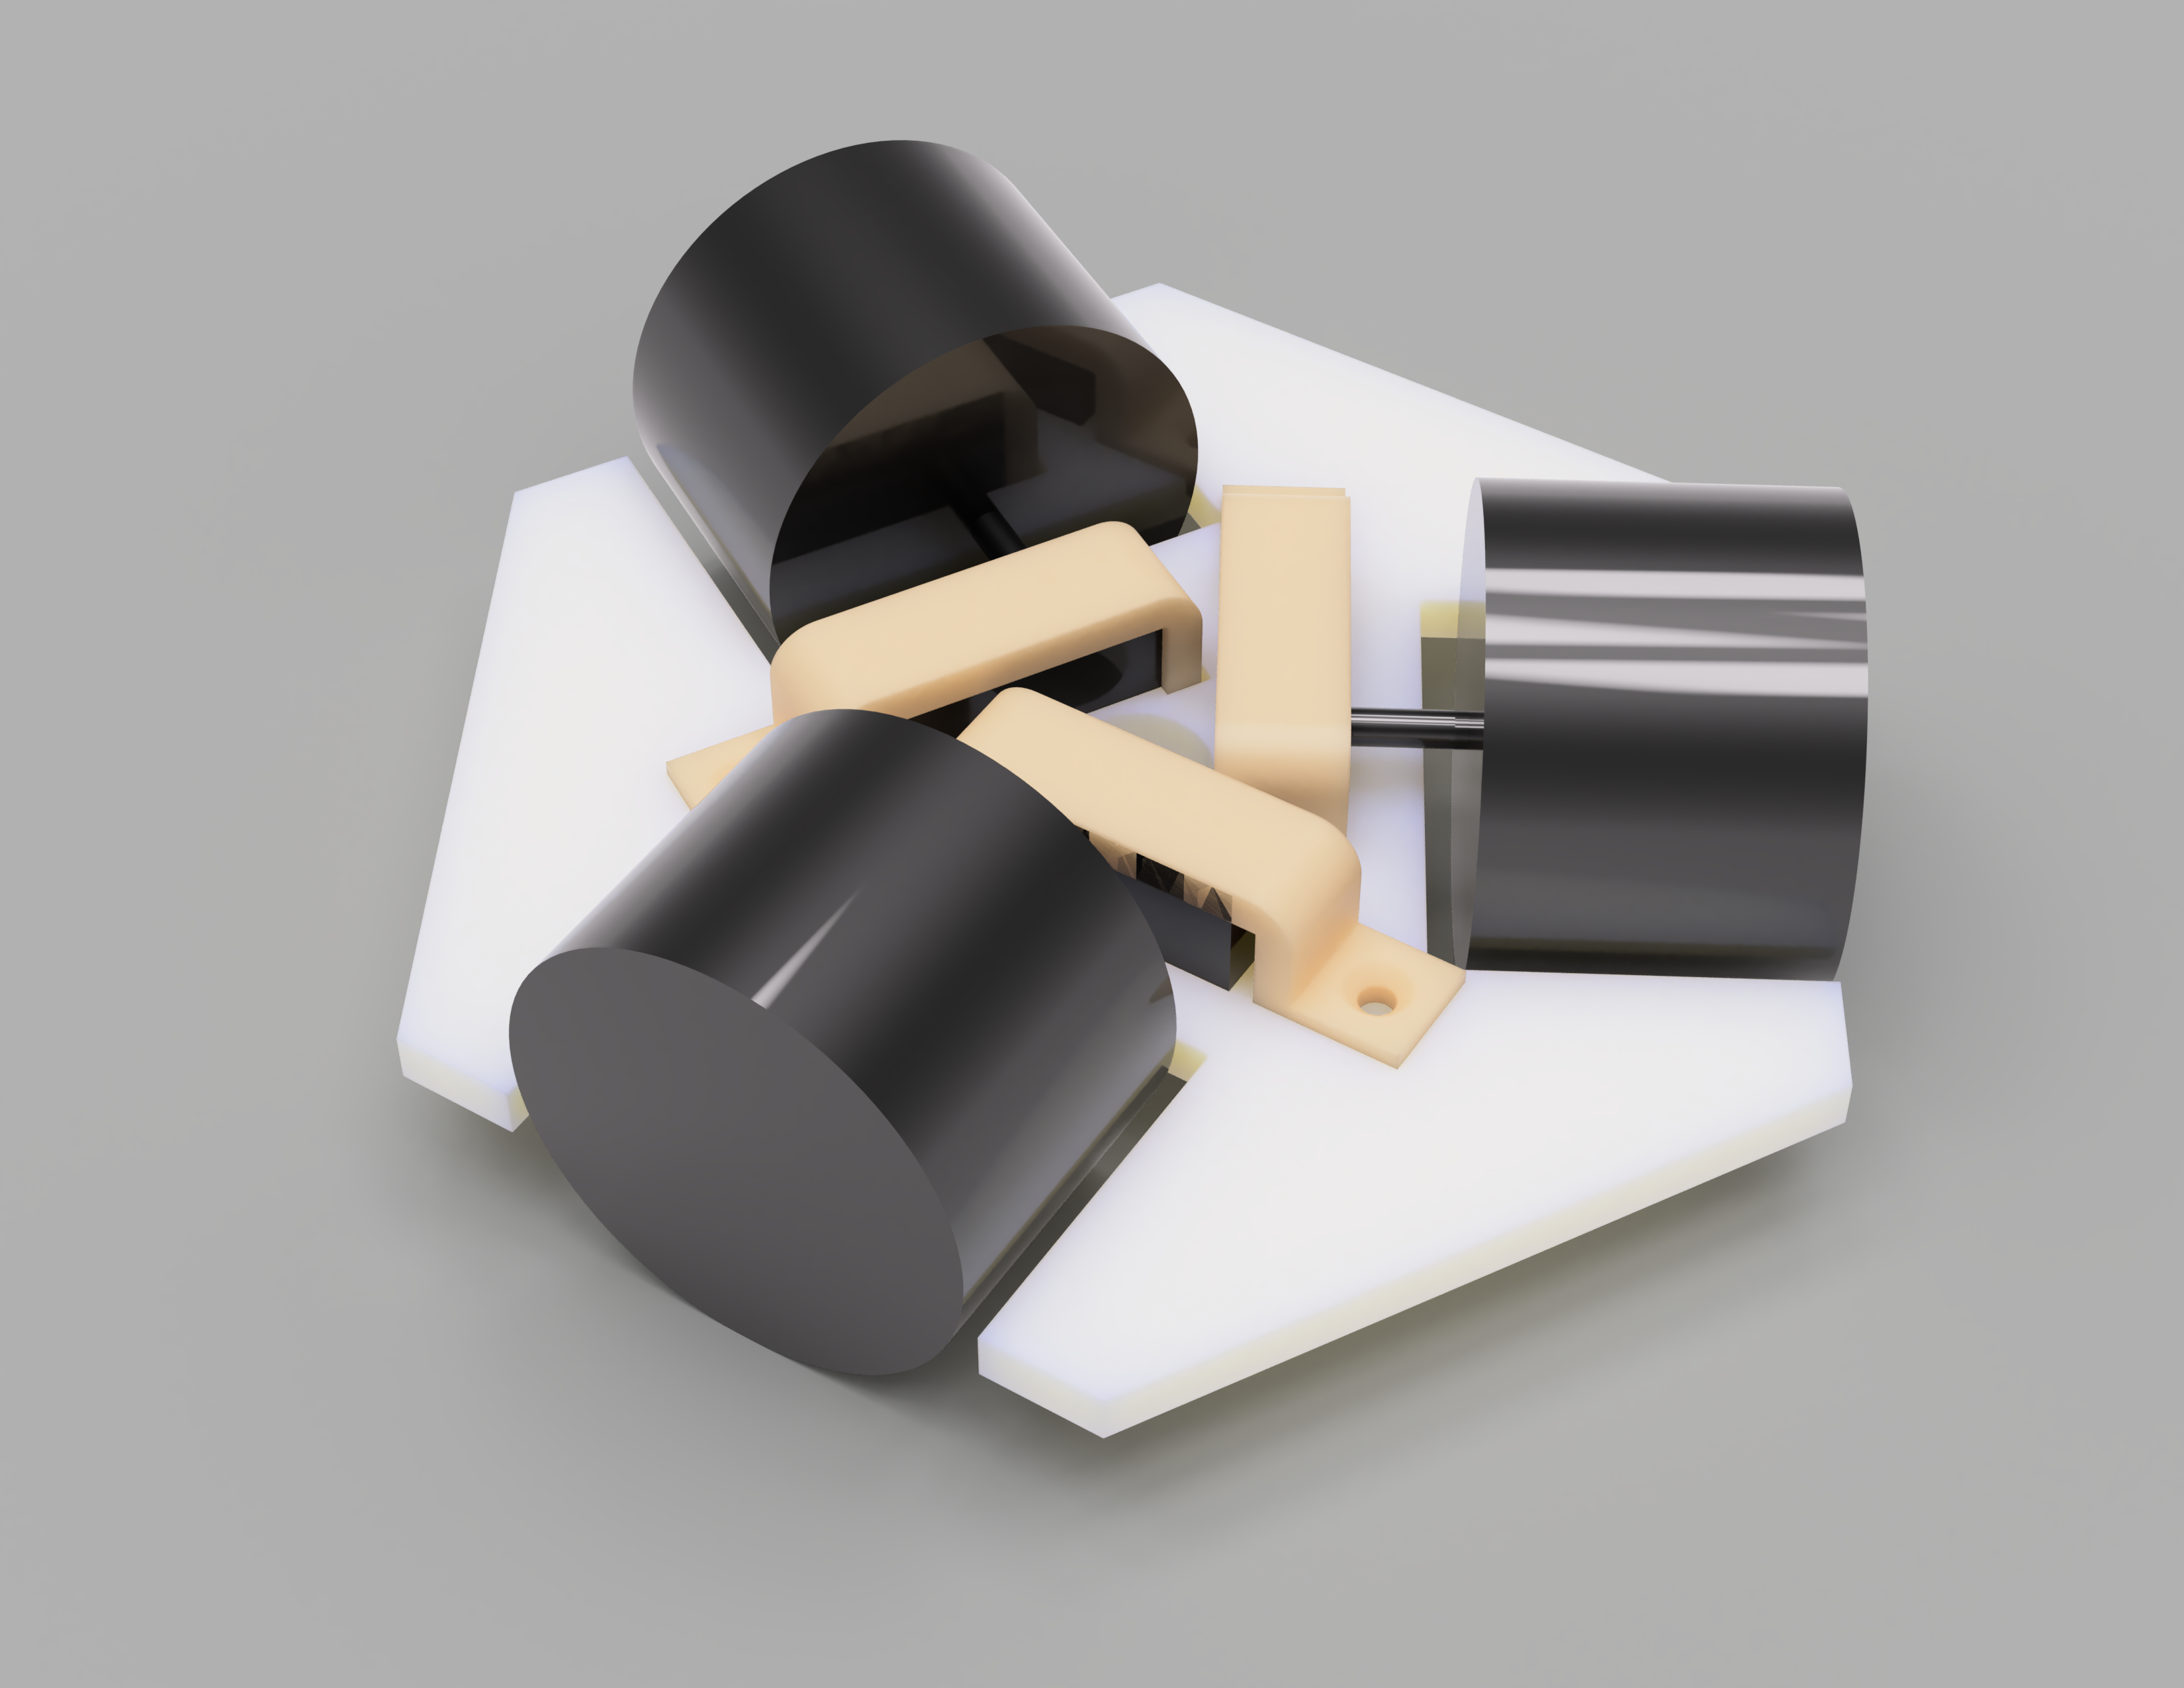
\includegraphics[width=\linewidth]{Assembled.png}
  \caption{Chassis render}
  \label{fig:ChassisRender}
\end{figure}

\begin{figure}[h]
  \centering
  \includegraphics[width=\linewidth]{Bottom-v3.jpg}
  \caption{The holonomic chassis}
  \label{fig:chassis}
\end{figure}

The commercial version's main circuit board is shown in Fig~\ref{fig:MainPCB}. The main processors onboard is an AVR microcontroller (Microchip ATmega2560-16AU) that combines 86 general-purpose I/O lines, 32 general purpose working registers, PWM, 4 USARTs, 16-channel 10-bit A/D converter, and a JTAG interface for on-chip debugging. ATmega2560 manages most logic computation.


\begin{figure}[h]
  \centering
  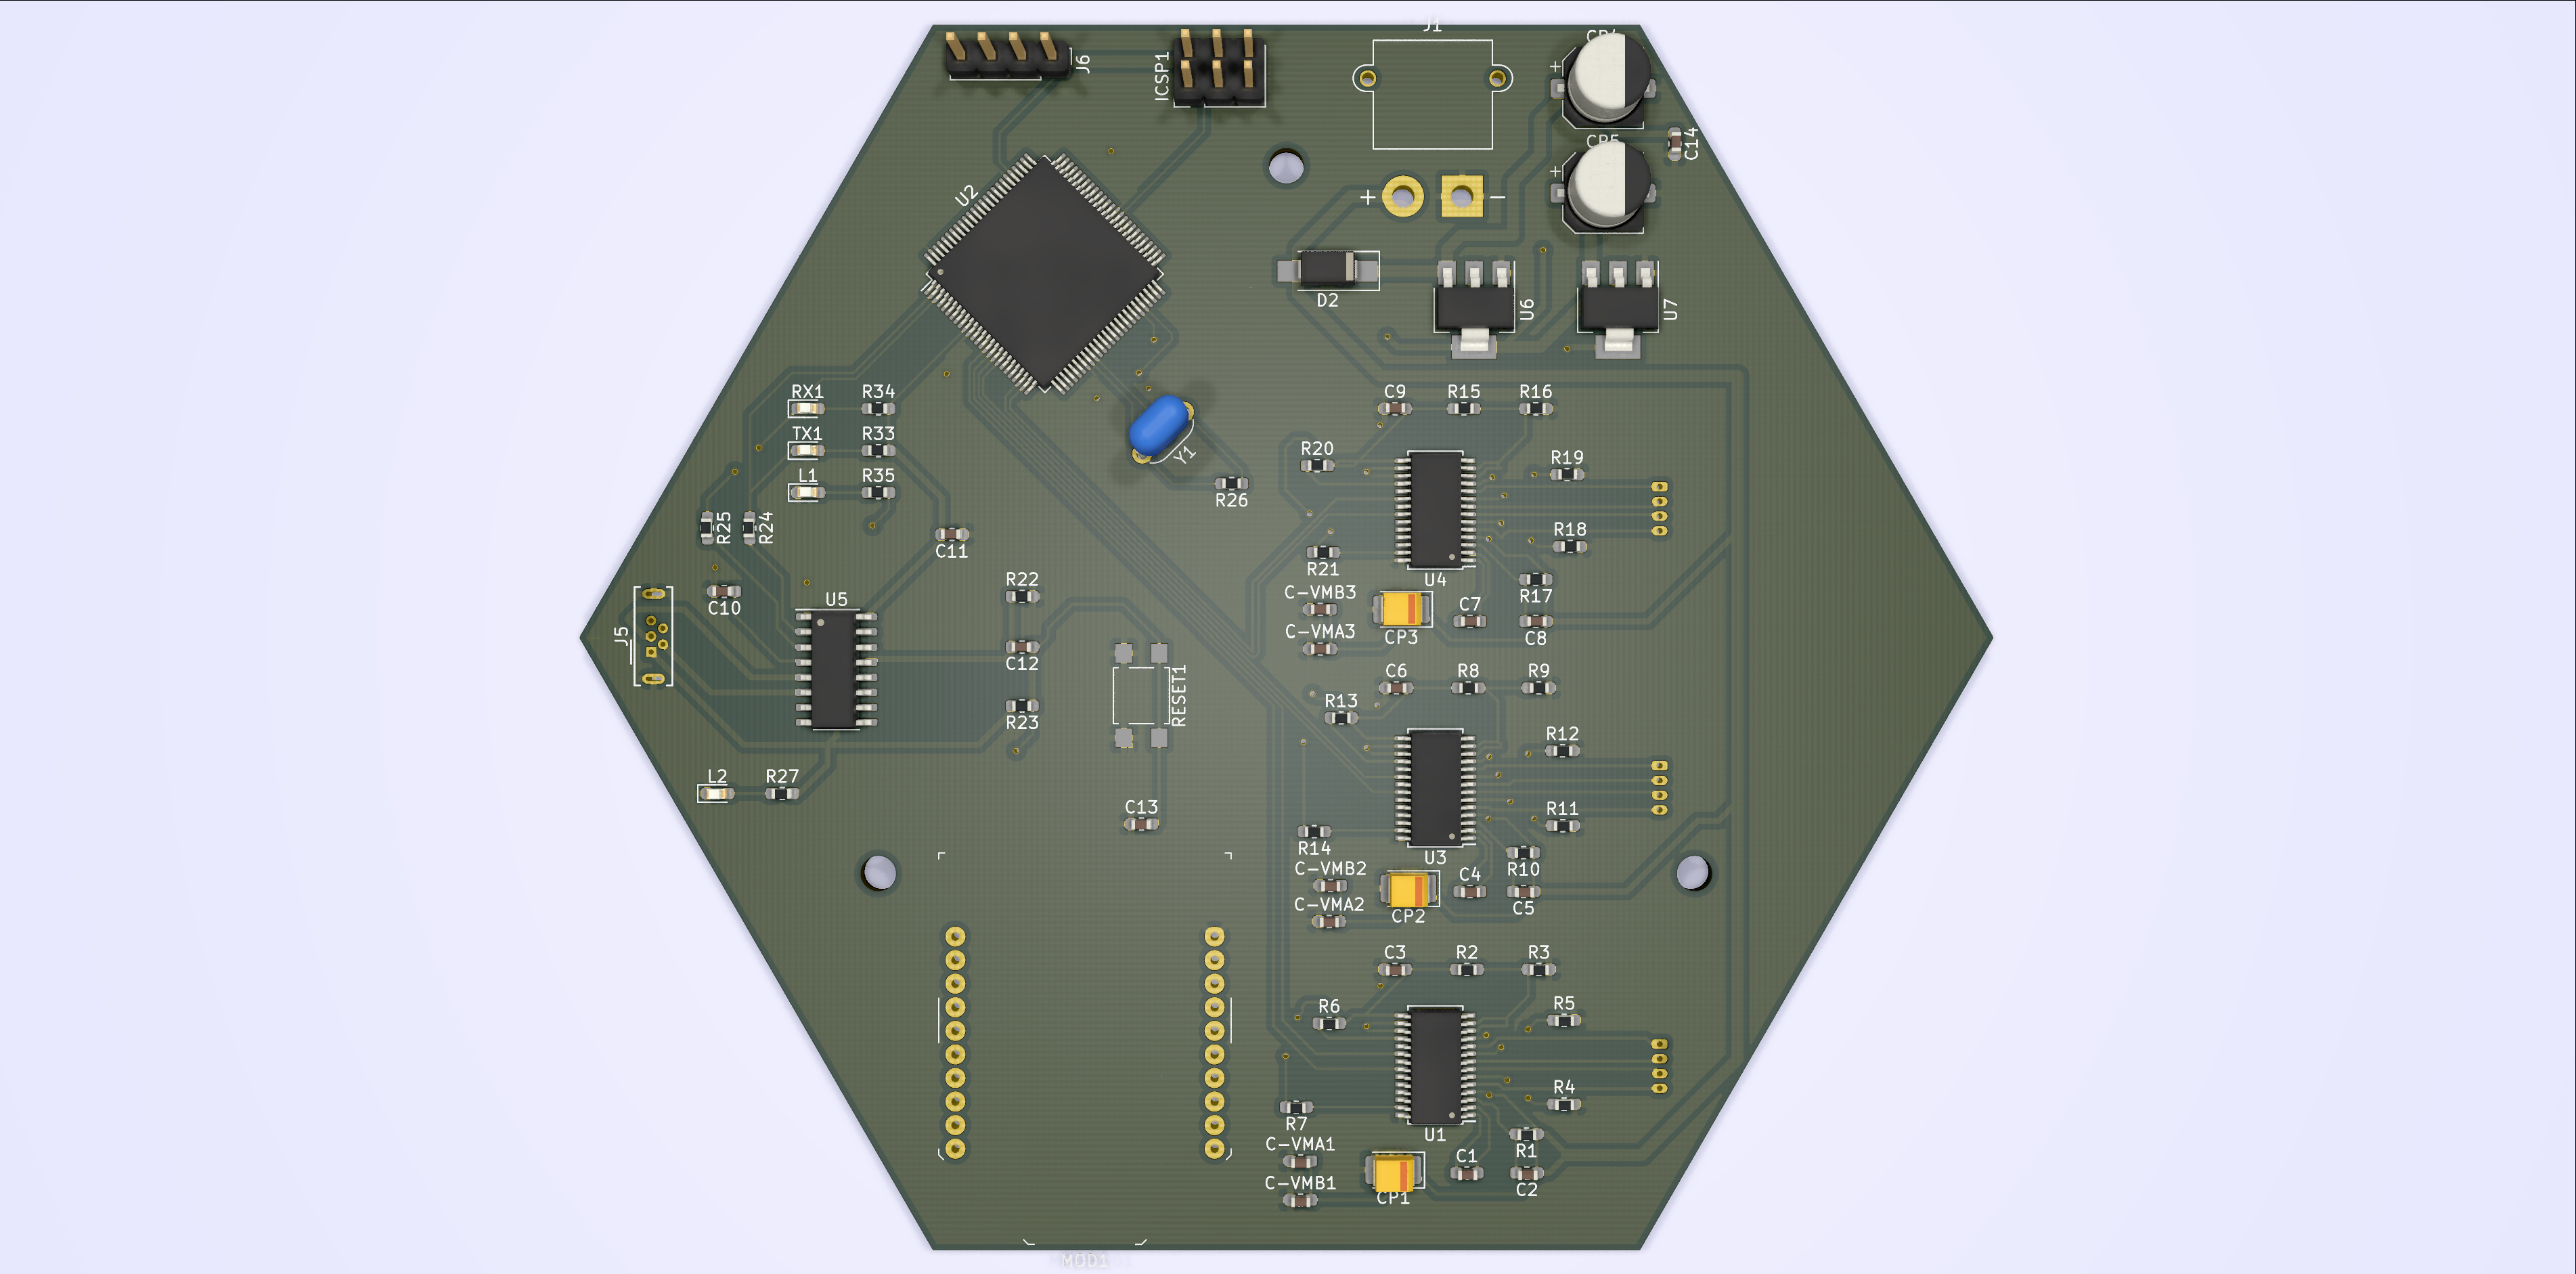
\includegraphics[width=\linewidth]{MainPCB.png}
  \caption{The commercial version PCB}
  \label{fig:MainPCB}
\end{figure}

% The PCB schematic is shown in Fig~\ref{fig:MainPCBschematic}, layout is shown in Fig~\ref{fig:MainPCBlayout}

% \begin{figure}[h]
%   \centering
%   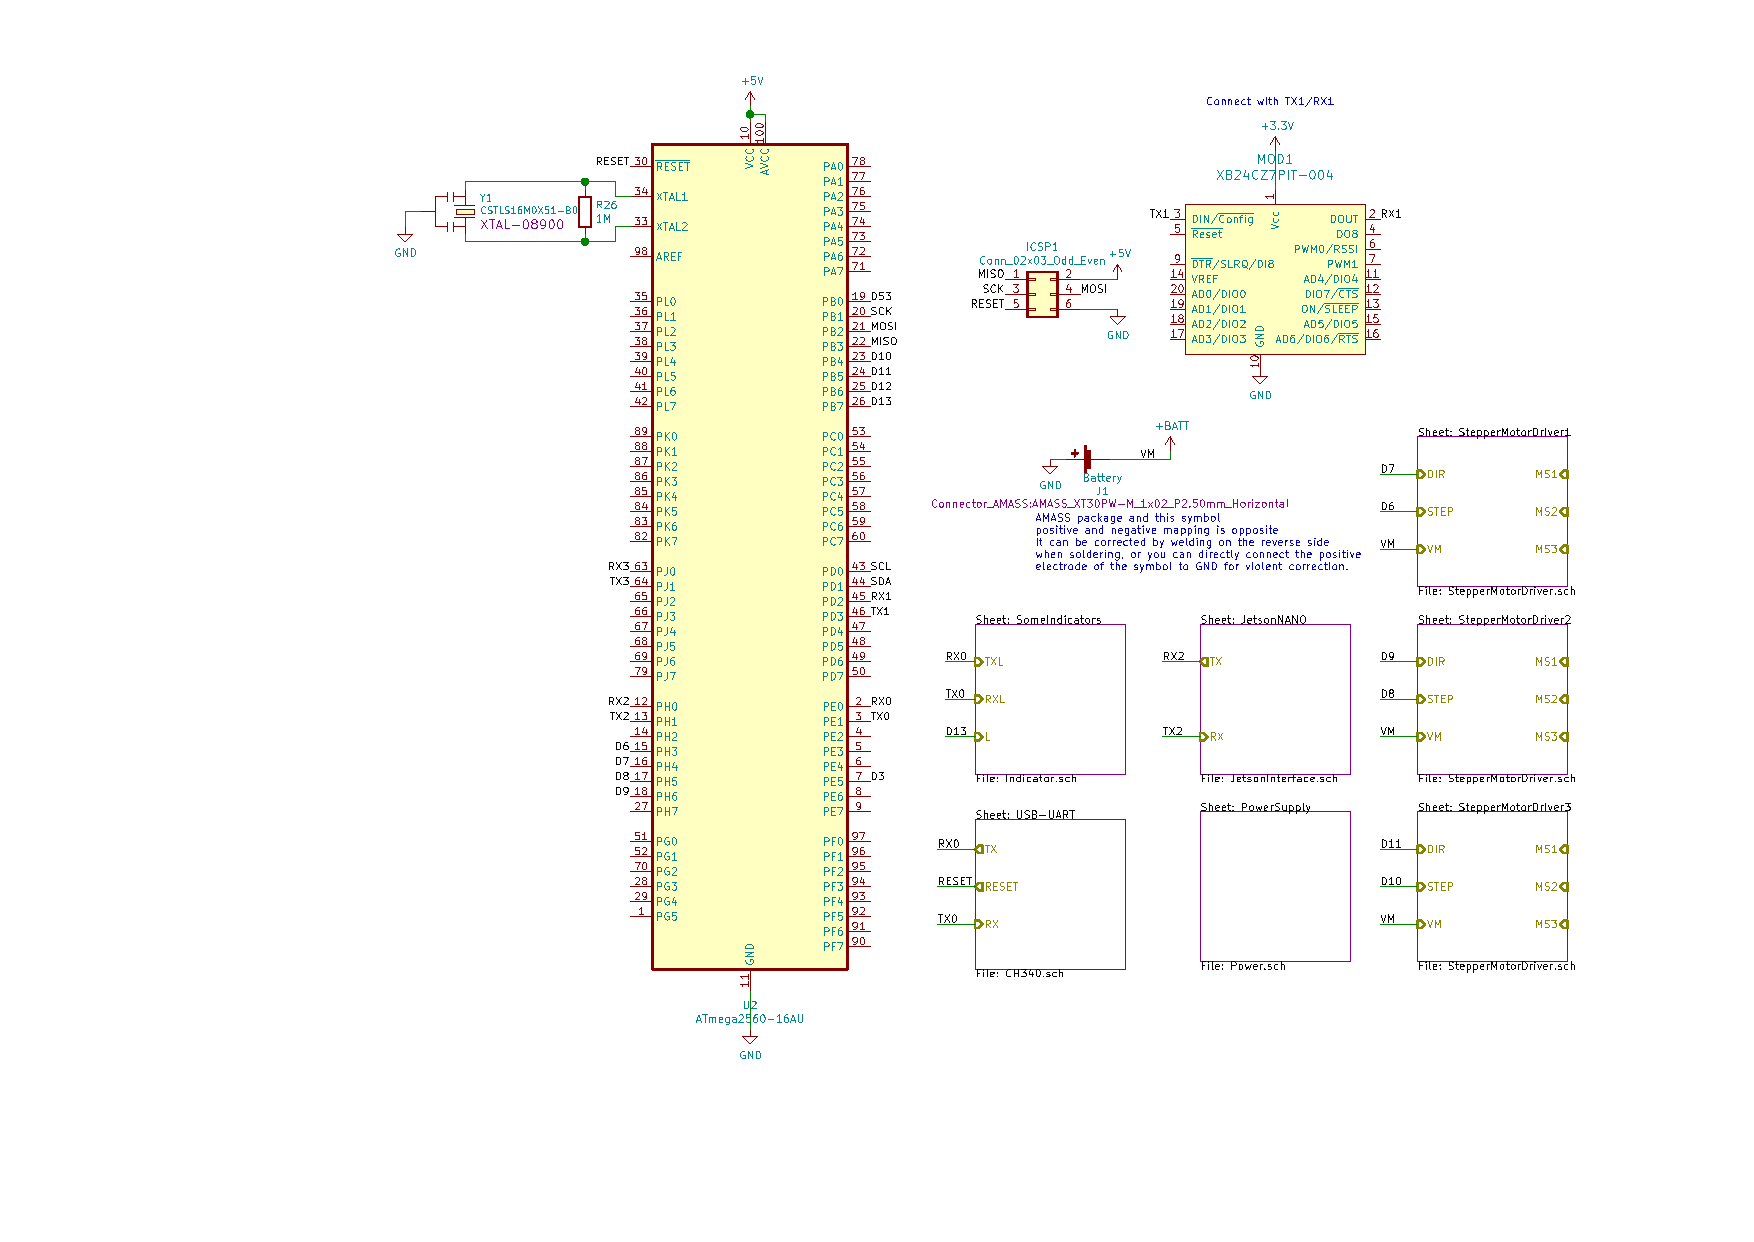
\includegraphics[width=\linewidth]{MisakaPCBv3-1.pdf}
%   \caption{The commercial version PCB schematic}
%   \label{fig:MainPCBschematic}
% \end{figure}

% \begin{figure}[h]
%   \centering
%   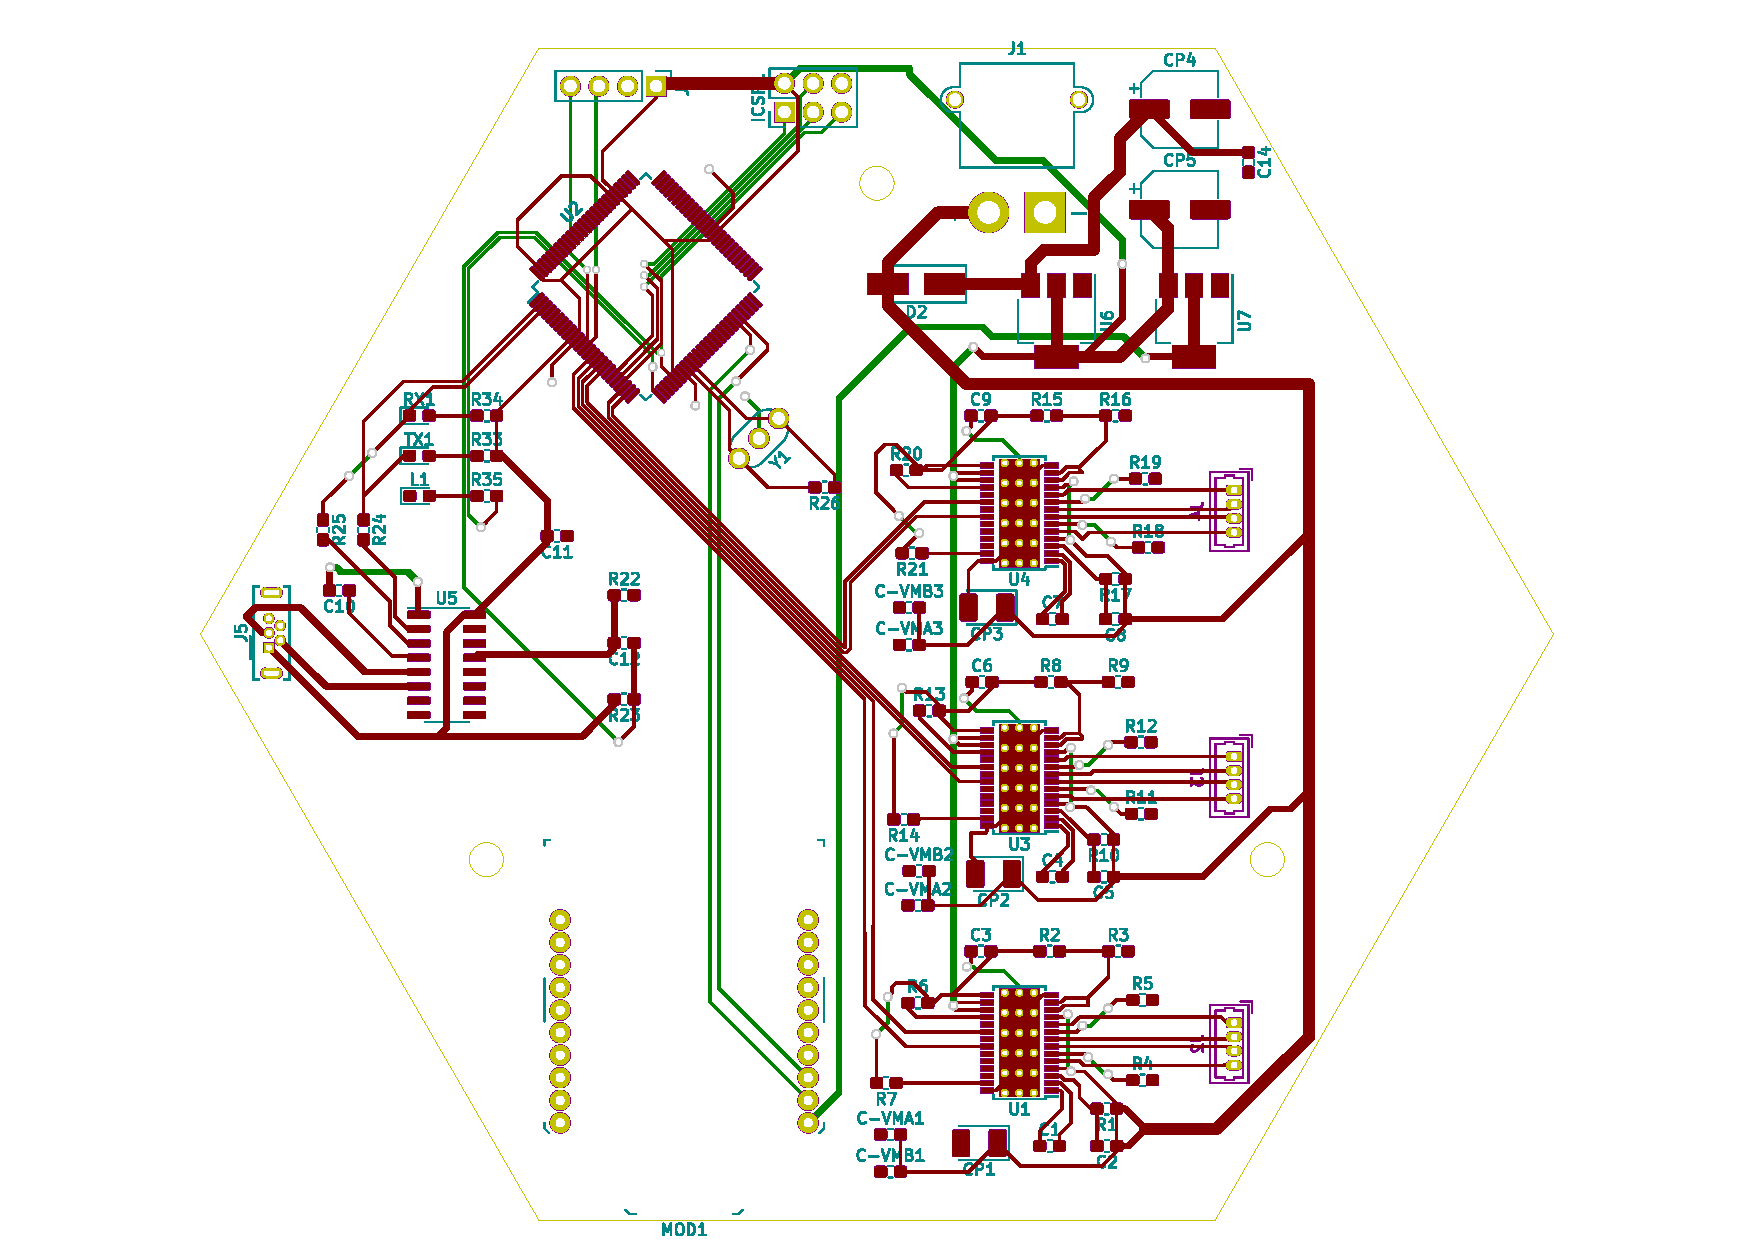
\includegraphics[width=\linewidth]{MisakaPCBv3-2.pdf}
%   \caption{The commercial version PCB layout}
%   \label{fig:MainPCBlayout}
% \end{figure}

Eight independently WS2812B LED on PCB illuminated in full RGB using are wrapped inside the 3D printed enclosure to provide the robot’s state display as well as full color indicating, shown in Fig~\ref{fig:RGB}.

\begin{figure}[h]
  \centering
  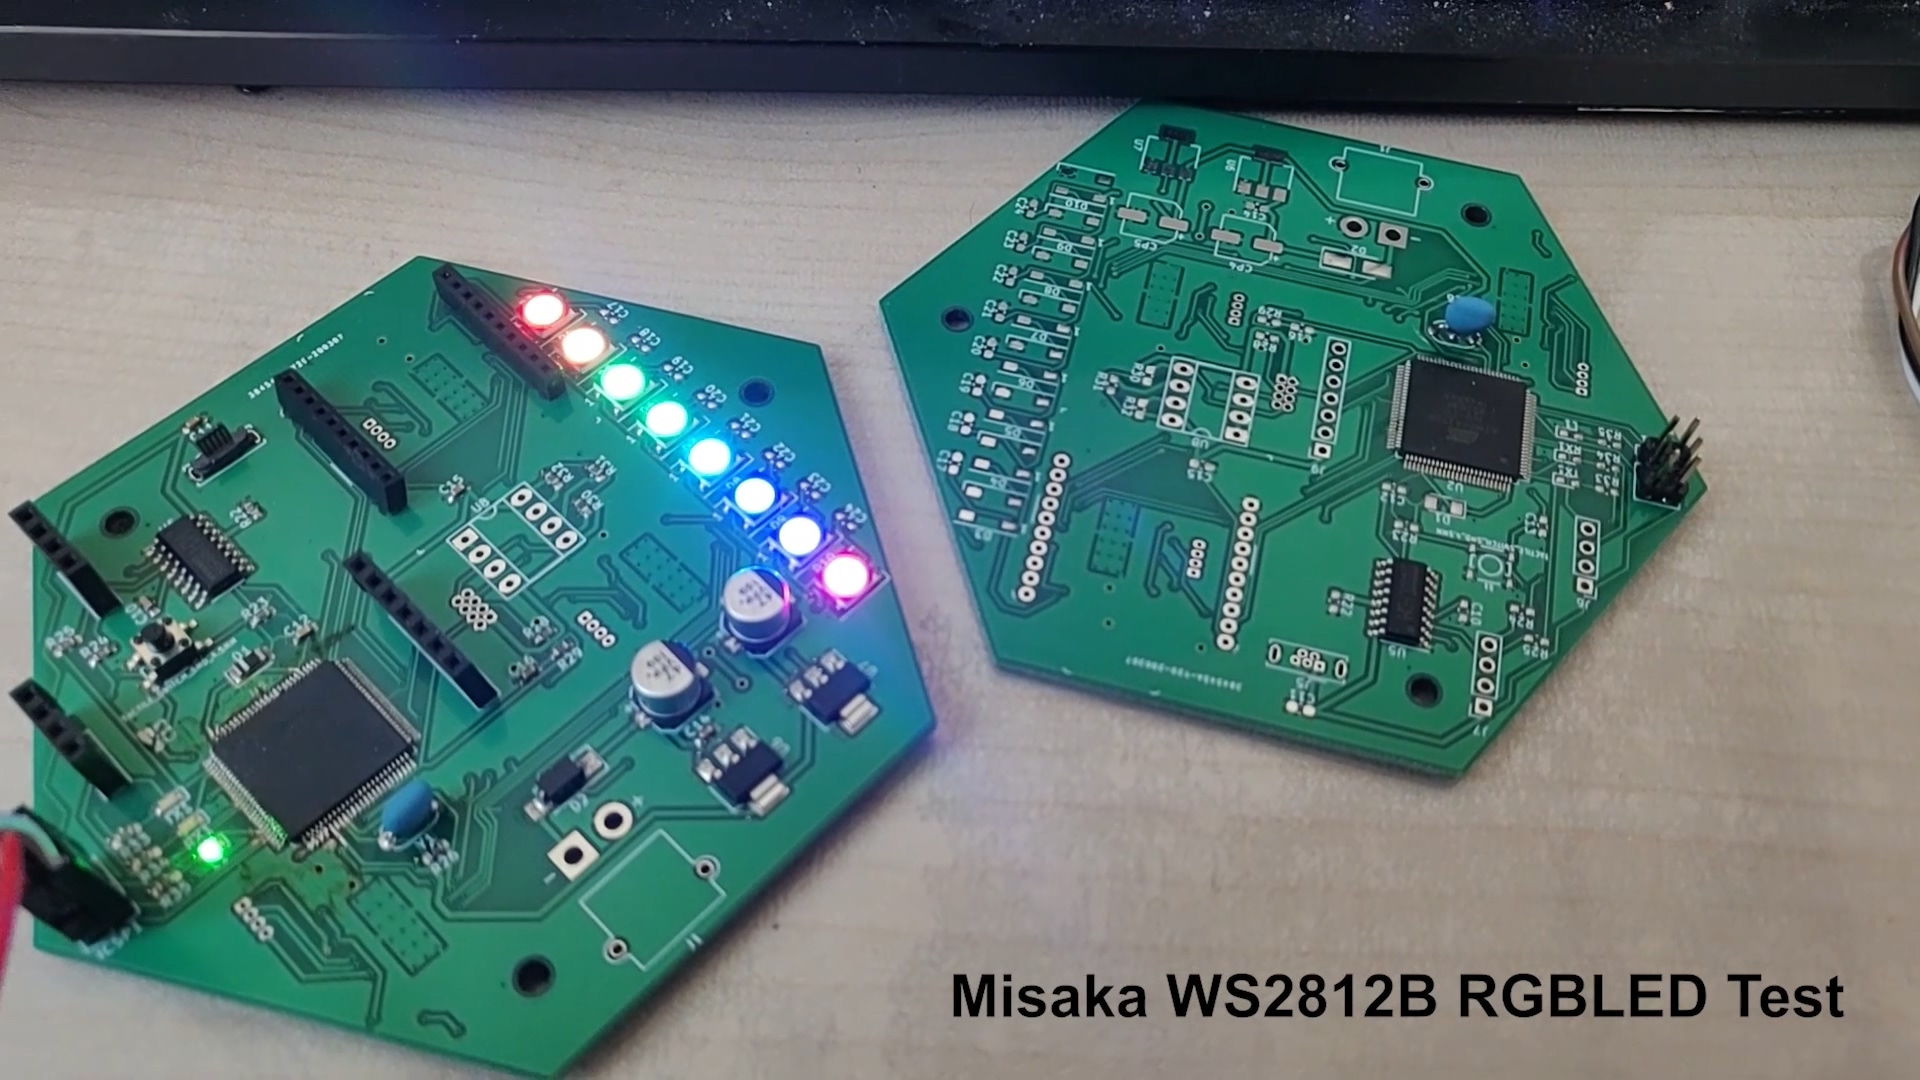
\includegraphics[width=\linewidth]{RGB.jpg}
  \caption{The RGB LED}
  \label{fig:RGB}
\end{figure}

Now robots communicate with each other using the Digi XBee module. XBee supports mesh networking which can be decentralized. We can use this feature to develop and test distributed algorithms that are also decentralized.

Users can modify the robot for their applications by designing custom modules that attach to its core module or adding powerful chips and development boards to achieve more functions, such as computer vision, wifi, machine learning algorithms, etc. Currently its compatible extensions are shown in Fig~\ref{fig:extensions}. For example, in order to give Misaka Linux development environment and capabilities of testing machine learning algorithms, we add Nvidia Jetson Nano to Misaka core through UART for high-level control and image processing. And to connect them with Bluetooth and wifi, we add ESP32 modules which also interact with Misaka through serial communication.\cite{zhang2020misaka}

\begin{figure}[h]
  \centering
  \includegraphics[width=\linewidth]{DA4A3991.JPG}
  \caption{Currently compatible extensions}
  \label{fig:extensions}
\end{figure}

\subsection{Explorer version}

For those researchers who want to develop distributed algorithms or tabletop swarm robots of their own, we provide an open-source PCB. 

It supports four kinds of different communication protocols, and integrates easy-to-use programmer and debug connector. To drive the stepper motor and DC motor, we have Powerstep01 on board with necessary components.
To extend its function, we provide a universal interface which can communicate with other development board such as Nvidia Jetson NANO.

All functionalities onboard are shown below:

\begin{itemize}
  \item Mega2560-16AU main MCU
  \item ATMega16U2 USB-UART
  \item USB Type C port
  \item PowerStep stepper motor and DC motor drive
  \item 9 x WS2812B RGB-LED full-color light display
  \item Downward looking infrared camera with dot paper for positioning
  \item XBee3, the main Mesh network communication
  \item Espressif ESP32, provides WiFi 5, Bluetooth, BLE communication
  \item CP2102. We can burn programs through the USB Type C port
  \item External battery power supply
  \item USB port power supply
  \item Buck DC-DC and impulse back pressure overvoltage and overcurrent protection
  \item Programmable pins for testing
  \item Support UART, I2C, SPI communication protocol expansion interface
\end{itemize}

% The PCB schematic is shown in Fig~\ref{fig:Explorer-schematic}, layout is shown in Fig~\ref{fig:Explorer-layout}, and its 3D model in Fig~\ref{fig:3Dmodel}. 
The PCB 3D model is shown in Fig~\ref{fig:3Dmodel}, After SMT, the PCB is shown in Fig~\ref{fig:PCBSMT}.

% \begin{figure}[h]
%   \centering
%   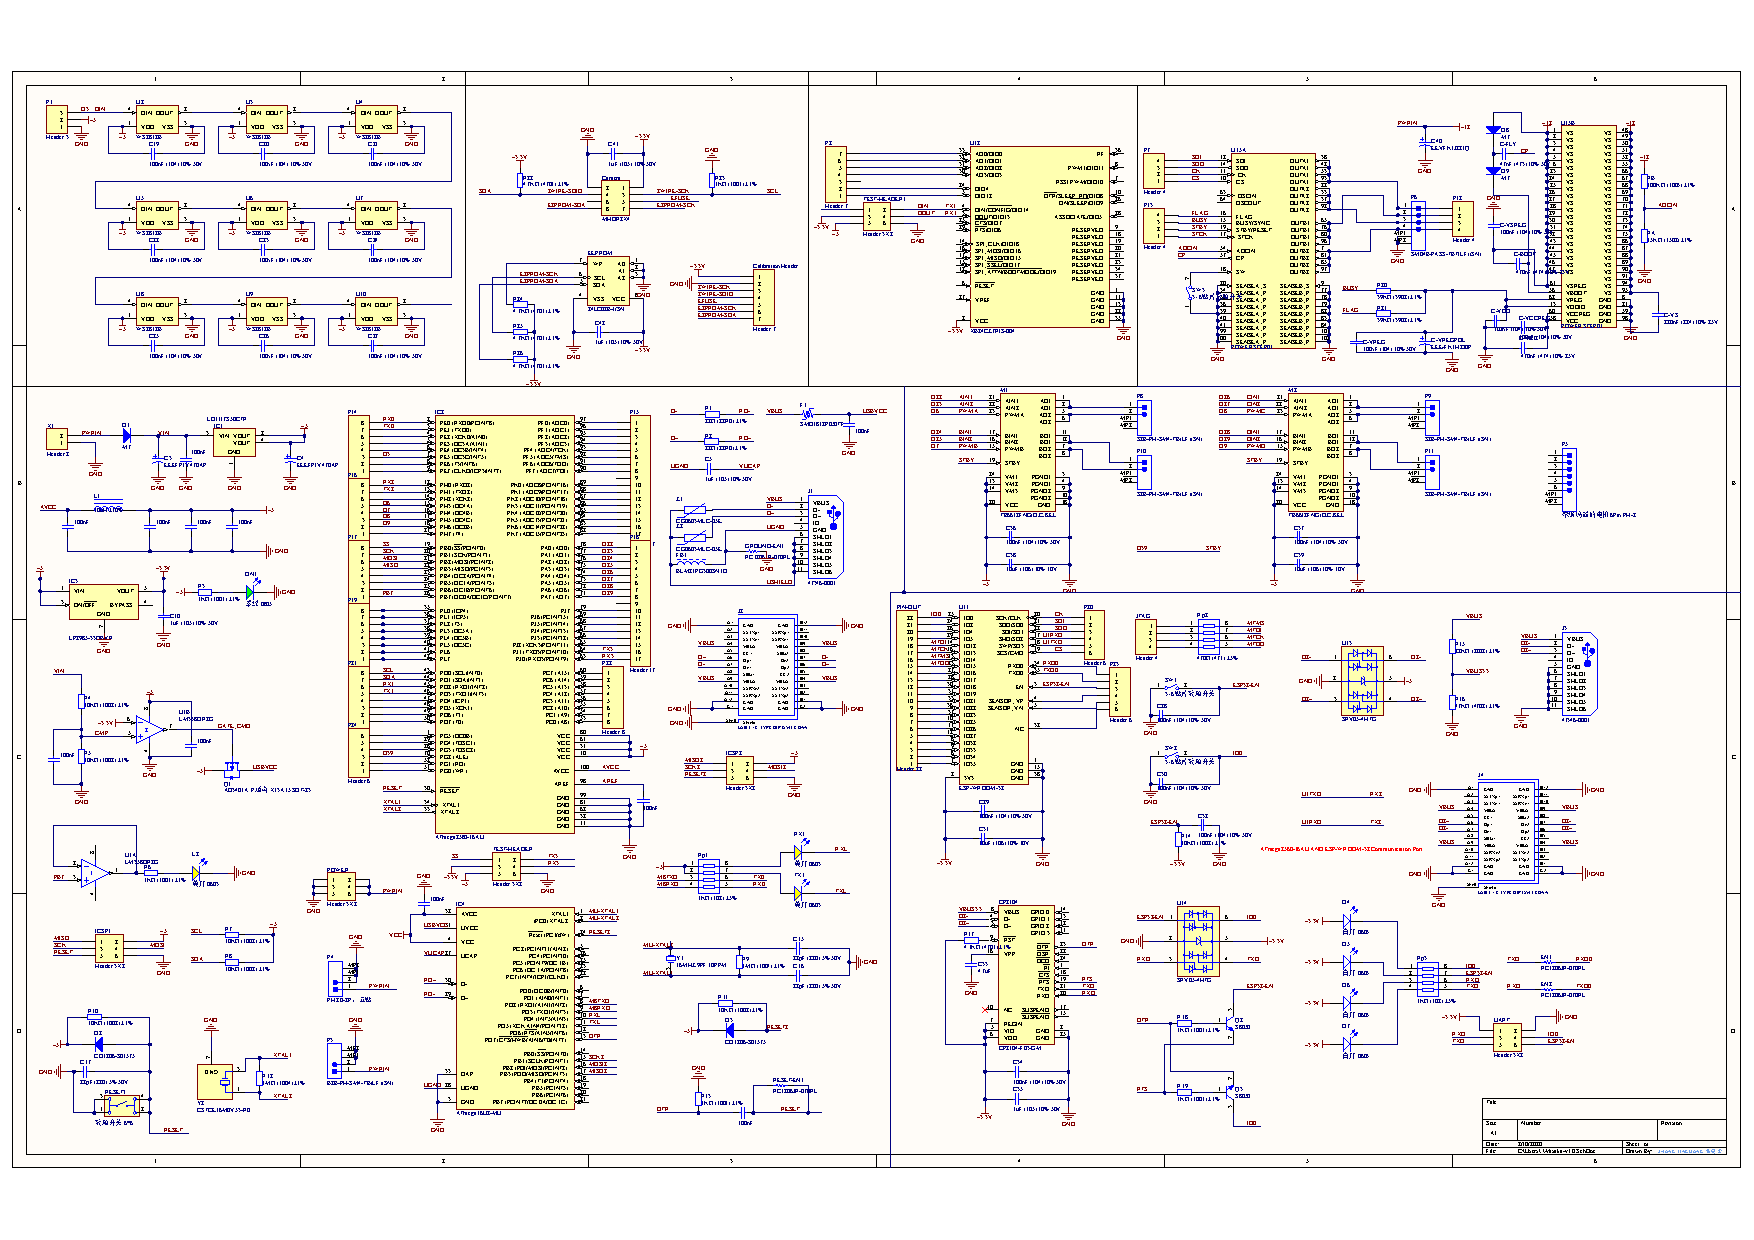
\includegraphics[width=\linewidth]{Misaka-v1-1.pdf}
%   \caption{Explorer version PCB schematic}
%   \label{fig:Explorer-schematic}
% \end{figure}


% \begin{figure}[h]
%   \centering
%   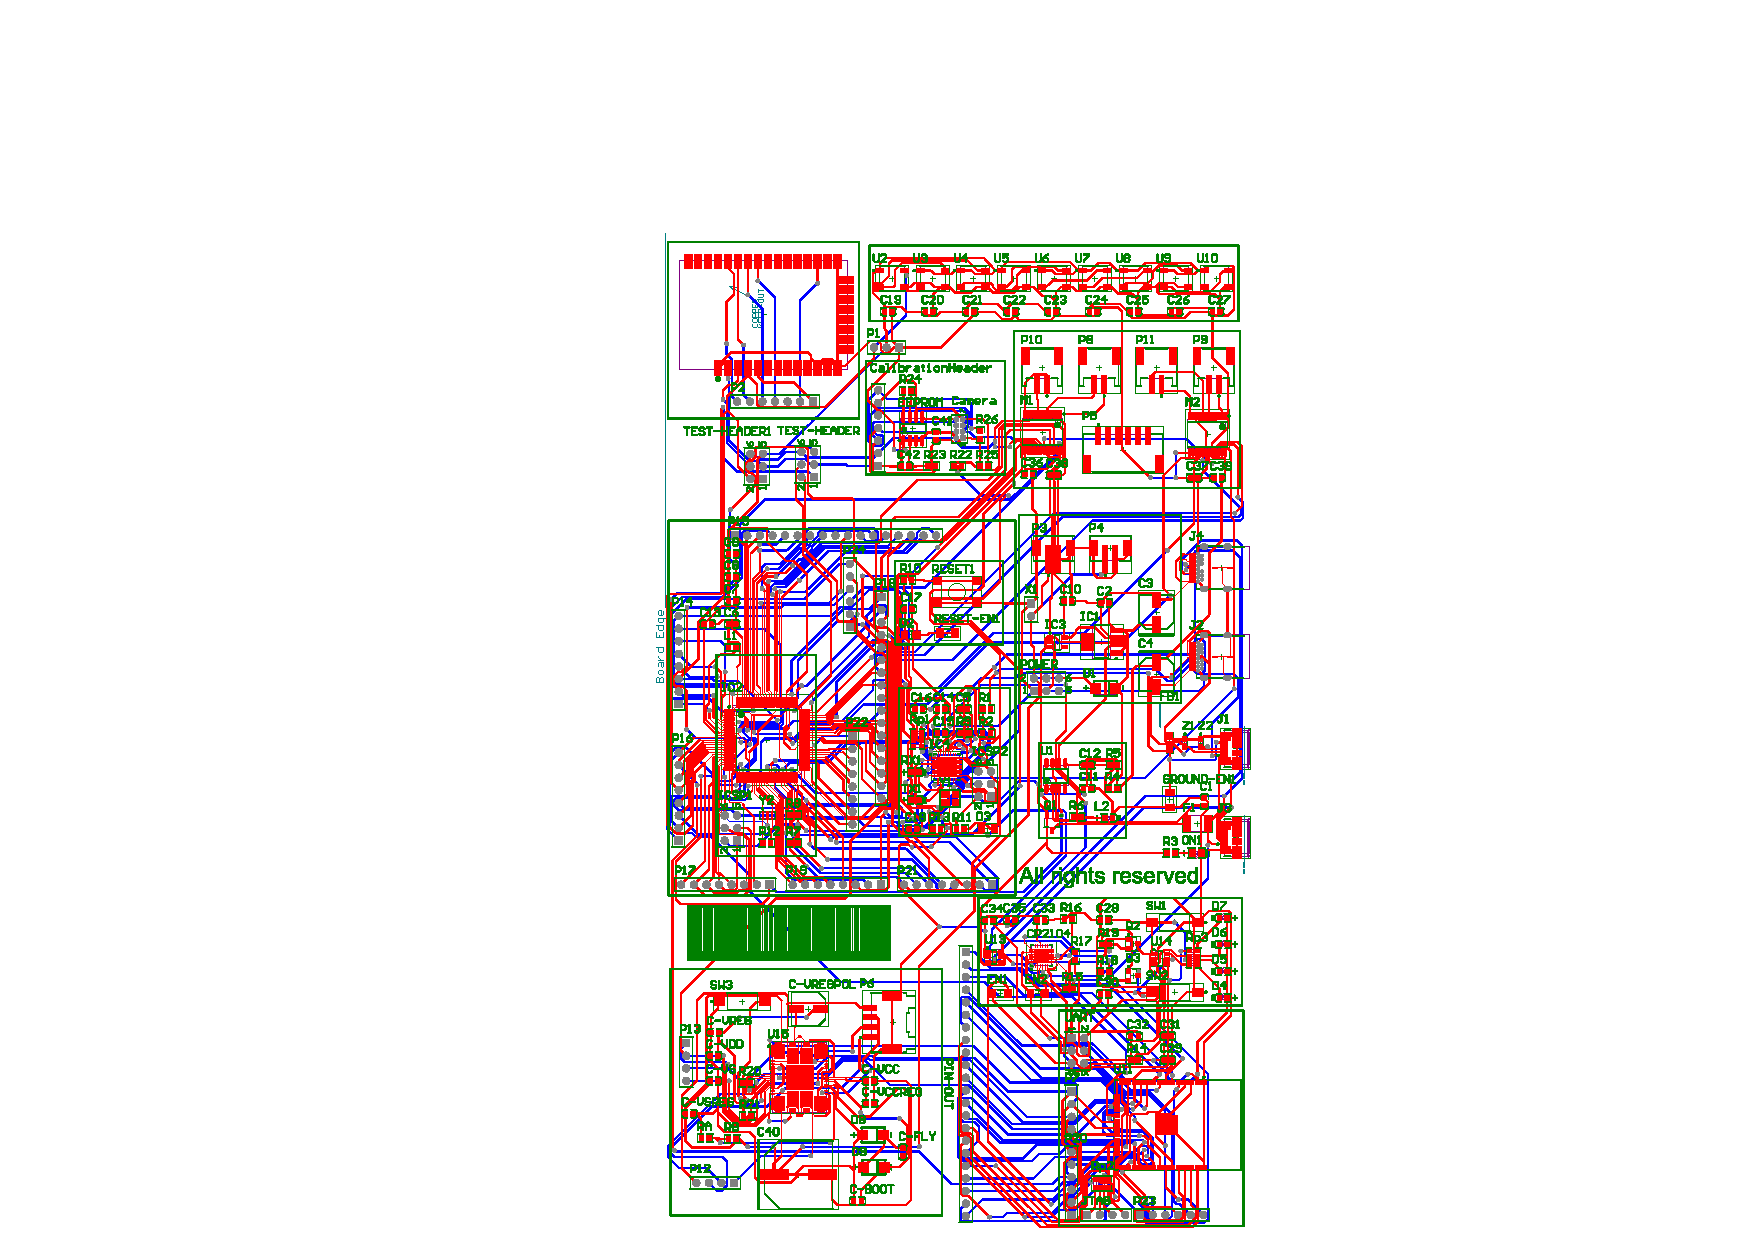
\includegraphics[width=\linewidth]{Misaka-v1-2.pdf}
%   \caption{Explorer version PCB layout}
%   \label{fig:Explorer-layout}
% \end{figure}

\begin{figure}[h]
  \centering
  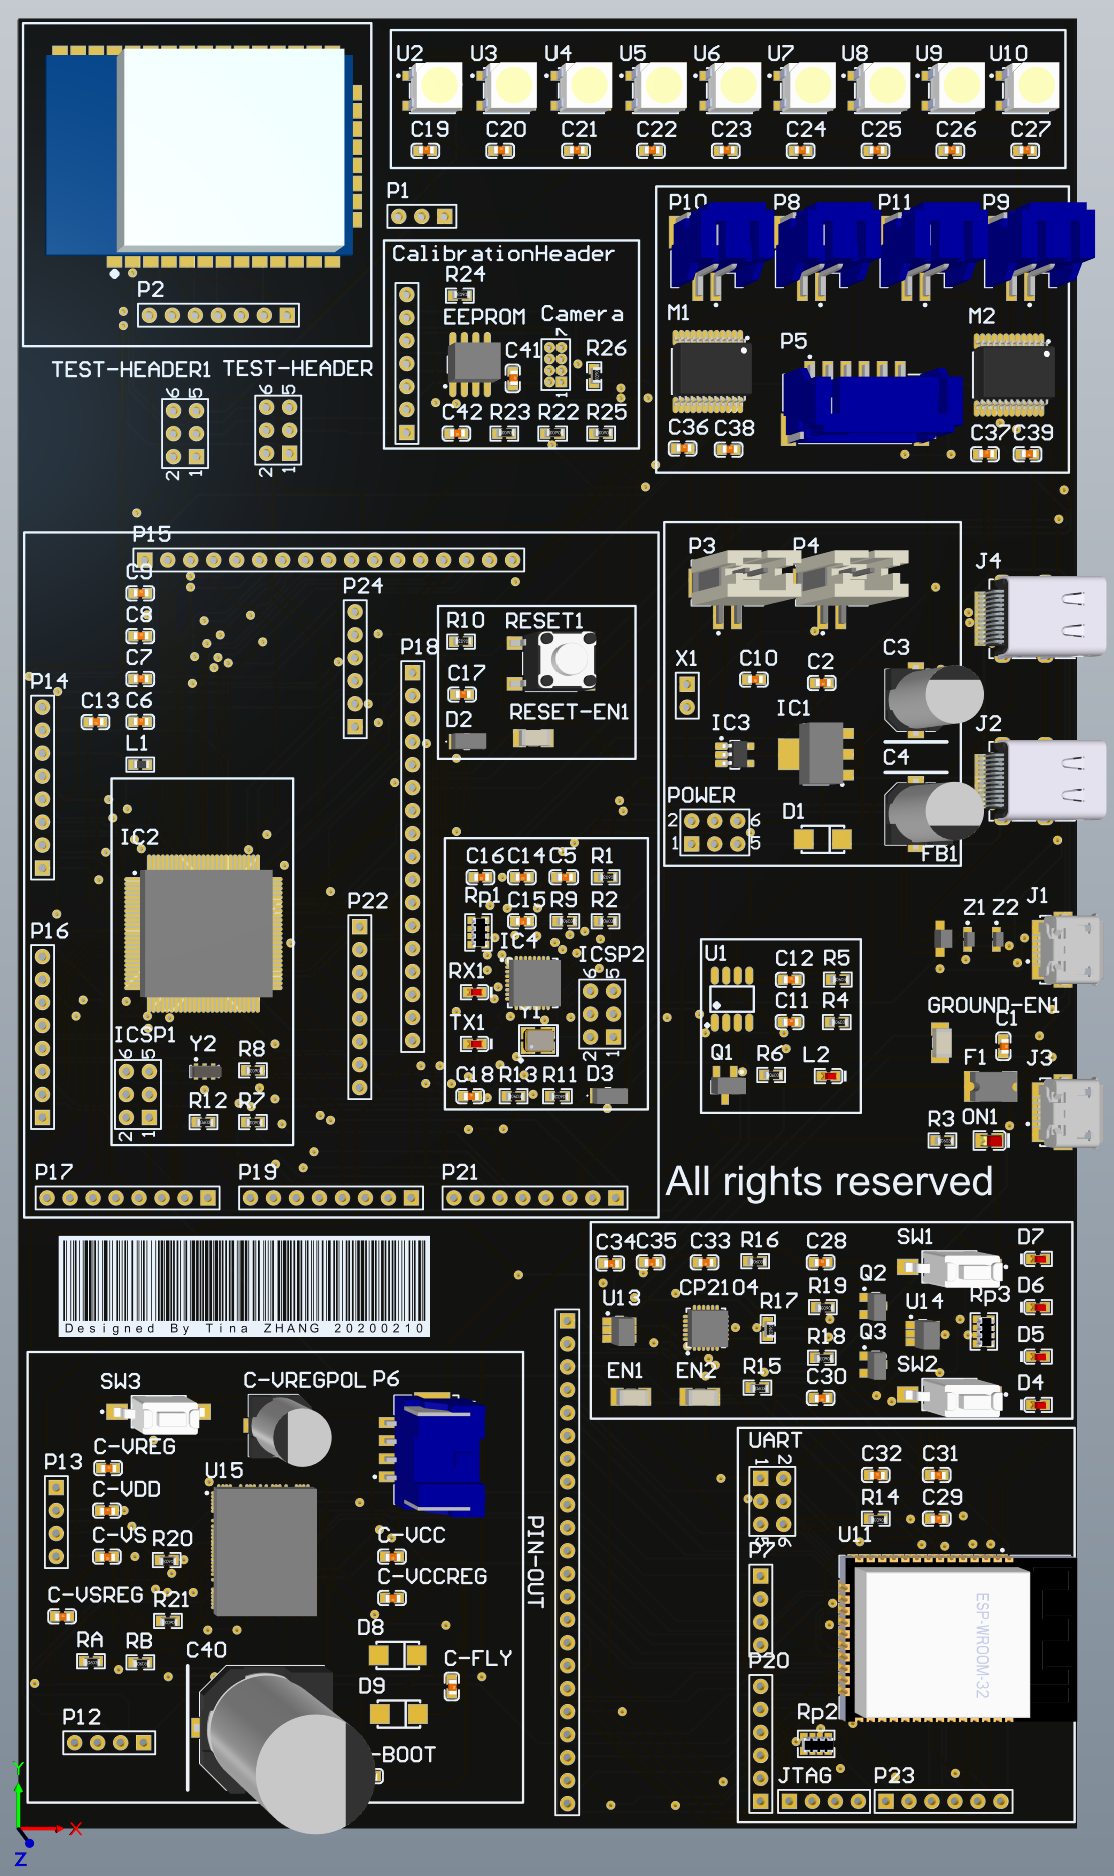
\includegraphics[width=\linewidth]{3DModel.png}
  \caption{3D model}
  \label{fig:3Dmodel}
\end{figure}

\begin{figure}[h]
  \centering
  \includegraphics[width=\linewidth]{TestBoard-SMT.jpg}
  \caption{PCB after SMT}
  \label{fig:PCBSMT}
\end{figure}

\section{Future RTLS with Bluetooth 5.1}

Real-time location systems (RTLS) are used to track and identify the location of objects in real-time using "Nodes" or "tags" attached to, or embedded in, the objects tracked, and "Readers" that receive and process the wireless signals from these tags to determine their locations.\cite{costs2009real}

The Bluetooth SIG presented Bluetooth 5.1 in January 2019. With Angle of Arrival (AoA) and Angle of Departure (AoD) which are used for location and tracking of devices, we can simply use BLE 5.1 as both communication and positioning methods.

Those techniques require one of the two communicating devices to have an array of multiple antennae, with the antenna array included in the receiving device when the AoA method is used and in the transmitting device when using AoD, as shown in Fig~\ref{fig:AODAOE}.\cite{woolley2019bluetooth}

With Bluetooth 5.1, we are able to track Misaka with a small margin of location error, as low as 10cm. The accuracy will be enough for many swarm applications.

\begin{figure}[h]
  \centering
  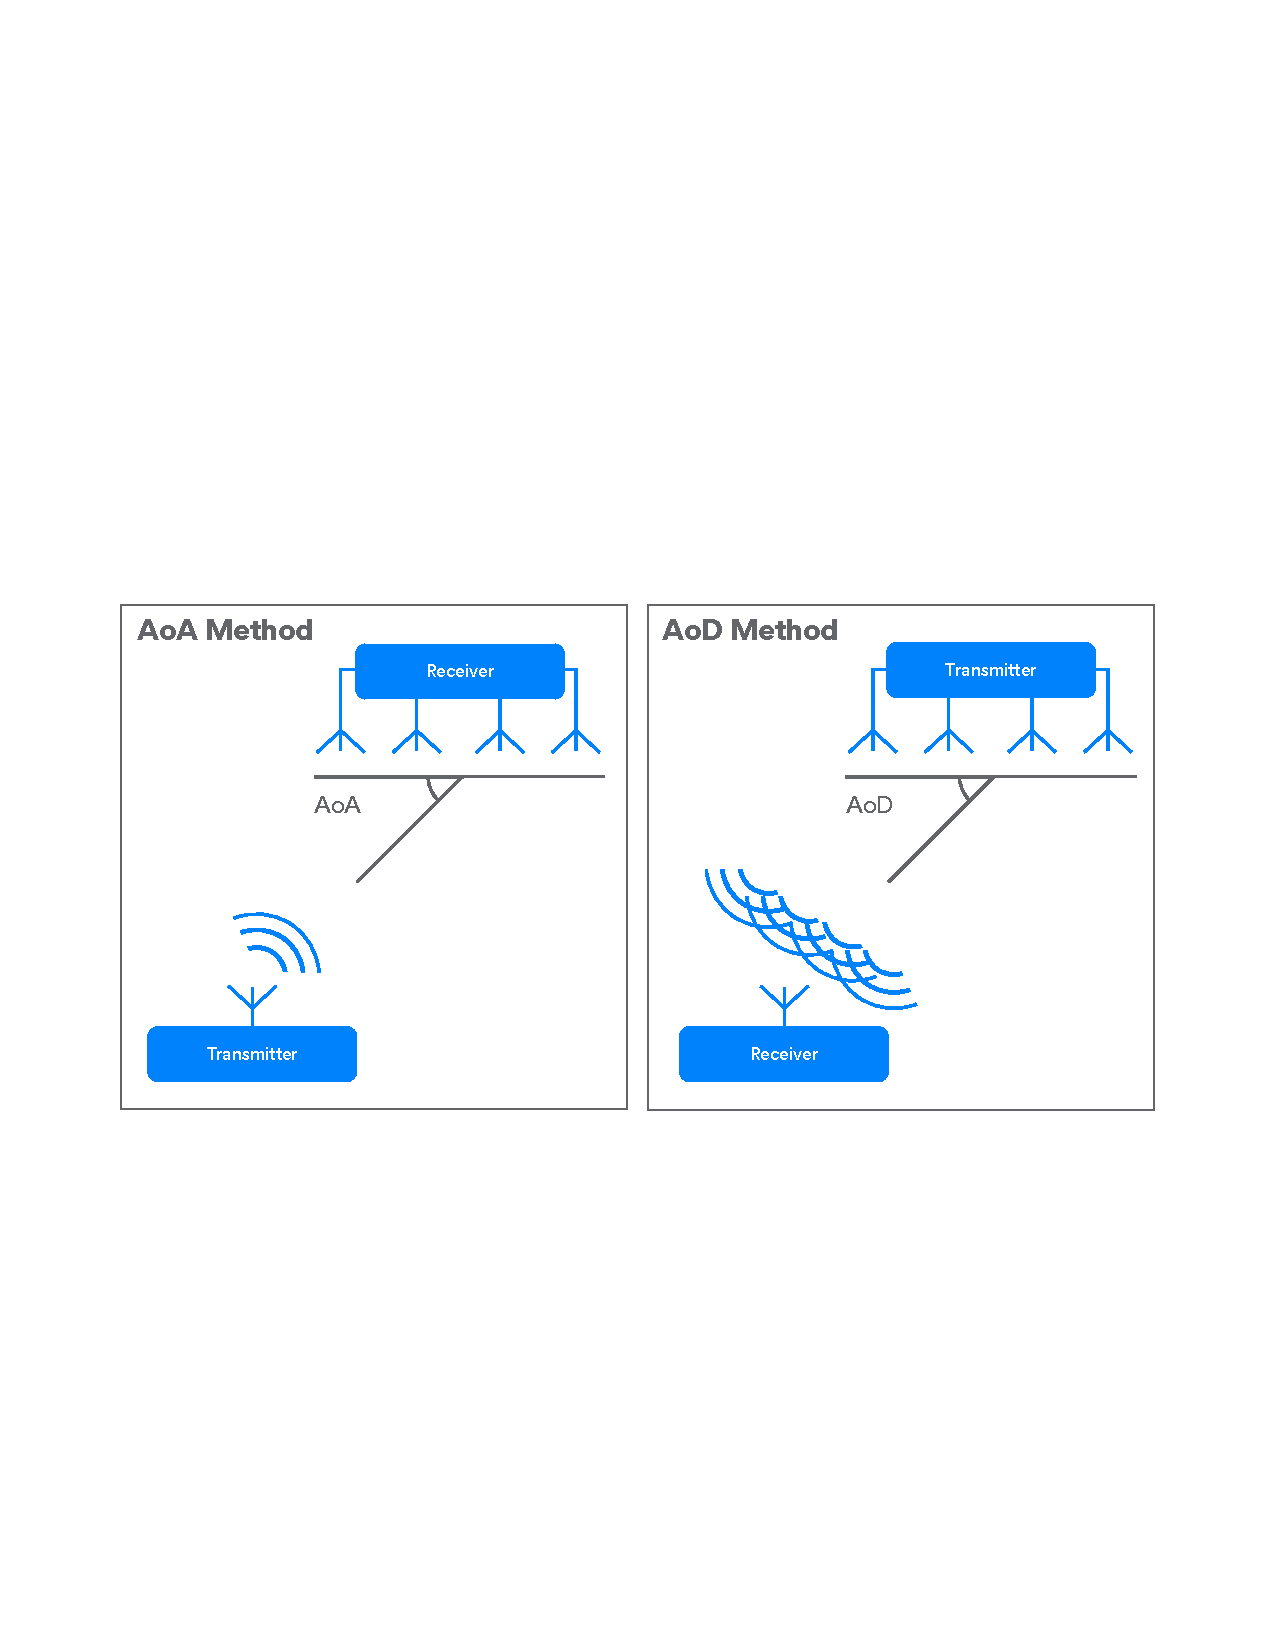
\includegraphics[width=\linewidth]{AODAOE.pdf}
  \caption{Angle of Arrival (AoA) and Angle of Departure (AoD)}
  \label{fig:AODAOE}
\end{figure}

\section{Conclusion}

We present Misaka, a versatile swarm robotics platform for swarm user interface development.

In summary, our contributions are:

\begin{itemize}
    \item The smallest omnidirectional open-source swarm platform.
    \item A set of scenarios to illustrate the possibilities offered by Misaka
    \item A common platform for any algorithm visualization, and other interactive swarm user interfaces
\end{itemize}

Furthermore, as benefits, Misaka:

\begin{itemize}
    \item are modular, can be extended with powerful platform.
    \item can simulate decentralized communication scenarios.
    \item are small enough to coexist in large numbers
    \item are relatively cost-effective: about 30 USD each now, down to \$10 if mass manufactured.
\end{itemize}

We hope that this paper and Misaka open-source platform will spur more research and creativity in the swarm user interface.

All necessary material and documentation for implementing Misaka can be found at Github.

%%
%% The acknowledgments section is defined using the "acks" environment
%% (and NOT an unnumbered section). This ensures the proper
%% identification of the section in the article metadata, and the
%% consistent spelling of the heading.
% \begin{acks}
% To my girlfriend, Yihan Jia, helping me during the research.
% \end{acks}

%%
%% The next two lines define the bibliography style to be used, and
%% the bibliography file.
\bibliographystyle{ACM-Reference-Format}
\bibliography{MisakaRef}

%%
%% If your work has an appendix, this is the place to put it.
% \appendix

\end{document}
\endinput
%%
%% End of file `sample-sigconf.tex'.
